\documentclass[a4paper]{article}
\usepackage[a4paper,margin=0mm]{geometry}
\usepackage{fontspec}
\usepackage{unicode-math}
\usepackage{tikz}
\usepackage[table]{xcolor}
\usepackage[absolute]{textpos}
\usepackage{array}
\usepackage{multirow}

\setmainfont{Libertinus Serif}
\setsansfont{Libertinus Sans}
\setmathfont{Libertinus Math}

\definecolor{accent}{HTML}{0F6A52}
\definecolor{badge}{HTML}{A9CFC2}
\definecolor{ink}{HTML}{2A2E30}

\setlength{\TPHorizModule}{1mm}
\setlength{\TPVertModule}{1mm}
\setlength{\parindent}{0pt}
\setlength{\parskip}{0pt}
\emergencystretch=3em
\abovedisplayskip=4pt plus 2pt minus 2pt \belowdisplayskip=4pt plus 2pt minus 2pt \abovedisplayshortskip=2pt \belowdisplayshortskip=2pt
\pagestyle{empty}

\newcommand{\LCOL}{16mm}
\newcommand{\RCOL}{111mm}
\newcommand{\COLW}{83mm}

\newcommand{\topicheader}[2]{%
\begin{textblock*}{194mm}(16mm,10mm)
\begin{tikzpicture}
\node[fill=accent,text=white,font=\sffamily\bfseries\fontsize{13}{13}\selectfont,
      minimum width=9mm,minimum height=9mm,inner sep=0pt] at (4.5mm,-4.5mm) {#1};
\node[font=\sffamily\bfseries\fontsize{15}{16}\selectfont,text=ink,anchor=west] at (12mm,-4.5mm) {#2};
\end{tikzpicture}
\end{textblock*}
\begin{textblock*}{194mm}(16mm,22.5mm)

\begin{tikzpicture}
\fill[accent] (0,0) rectangle (194mm,0.5mm);
\end{tikzpicture}
\end{textblock*}
}

\newcommand{\pagefooter}[1]{%
\begin{textblock*}{194mm}(8mm,286.41mm)
  
\begin{tikzpicture}
    \fill[accent] (0,0) rectangle (194mm,0.6mm);
  \end{tikzpicture}
\end{textblock*}
\begin{textblock*}{63.59mm}(8mm,288.27mm)
  {\sffamily\bfseries\color{accent}\fontsize{13}{16}\selectfont SAT 1200+}
\end{textblock*}
\begin{textblock*}{10mm}(188mm,288.27mm)
  \centering{\sffamily\color{accent}\fontsize{14}{16}\selectfont #1}
\end{textblock*}
}

\newcommand{\colrule}[2]{%
\begin{textblock*}{1mm}(105mm,#1mm)
\begin{tikzpicture}
\draw[black!65,line width=0.5pt] (0,0) -- (0,#2mm);
\end{tikzpicture}
\end{textblock*}
}

\newcommand{\setkicker}[2]{%
{\sffamily\bfseries\fontsize{12}{14}\selectfont #1.}\ {\itshape\fontsize{11}{14}\selectfont\color{black!75} #2}\par\vspace{2mm}%
}

\setlength{\fboxsep}{1.4pt}
\setlength{\fboxrule}{0.5pt}
\newcommand{\pnum}[1]{\fcolorbox{ink}{white}{\sffamily\bfseries\fontsize{8}{8}\selectfont #1}~}

% ---- SAT-style multiple-choice block (2x2 grid of short choices) ----
\newcommand{\satq}[6]{%
\noindent\pnum{#1} #2\par\nobreak\vspace{2mm}%
\noindent\hspace*{7mm}\begin{tabular}[t]{@{}p{32mm}p{32mm}@{}}
(A) #3 & (B) #4 \\[2mm]
(C) #5 & (D) #6 \\
\end{tabular}\par\vspace{5.5mm}%
}

% ---- stacked choices for long ones ----
\newcommand{\satqw}[6]{%
\noindent\pnum{#1} #2\par\nobreak\vspace{2mm}%
\noindent\hspace*{7mm}(A) #3\par\vspace{1.6mm}%
\noindent\hspace*{7mm}(B) #4\par\vspace{1.6mm}%
\noindent\hspace*{7mm}(C) #5\par\vspace{1.6mm}%
\noindent\hspace*{7mm}(D) #6\par\vspace{5.5mm}%
}

% ---- student-produced response (grid-in) ----
\newcommand{\satg}[2]{%
\noindent\pnum{#1} {\sffamily\bfseries\fontsize{7}{8}\selectfont\color{accent}GRID-IN}\ #2\par\nobreak\vspace{2.5mm}%
\noindent\hspace*{7mm}{\sffamily\fontsize{8.5}{10}\selectfont Answer:}\ \rule[-1.2mm]{28mm}{0.4pt}\par\vspace{5.5mm}%
}

% ---- worked-solution entry ----
\newcommand{\solitem}[4]{%
\noindent\pnum{#1} {\bfseries #2}\ —\ #3\ {\itshape\color{accent}[#4]}\par\vspace{2.1mm}%
}

\usetikzlibrary{arrows.meta}
\newsavebox{\figsave}
\newcommand{\figbox}[1]{\par\vspace{1.8mm}\sbox{\figsave}{#1}\noindent\hfill\ifdim\wd\figsave>\hsize\resizebox{\hsize}{!}{\usebox{\figsave}}\else\usebox{\figsave}\fi\hfill\null\par\vspace{0.8mm}}
\arrayrulecolor{accent}
\setlength{\arrayrulewidth}{0.7pt}
\renewcommand{\arraystretch}{1.3}

\usepackage{multicol}
\usepackage{fancyhdr}
\usepackage{needspace}
\newcommand{\pgoff}{0}
\renewcommand{\solitem}[4]{\noindent\parbox[t]{\linewidth}{\raggedright\pnum{#1} {\bfseries #2}\ ---\ #3\ {\itshape\color{accent}[#4]}}\par\vspace{3.6mm}}
\newcommand{\solkicker}[2]{\Needspace{38mm}\vspace{1.5mm}{\sffamily\bfseries\fontsize{12.5}{15}\selectfont #1.}\ {\itshape\fontsize{11}{14}\selectfont\color{black!75} #2}\par\vspace{3mm}}
\renewcommand{\satqw}[6]{%
\noindent\pnum{#1} #2\par\nobreak\vspace{2mm}%
\noindent\hangindent=13mm\hangafter=1\hspace*{7mm}(A)~#3\par\vspace{1.6mm}%
\noindent\hangindent=13mm\hangafter=1\hspace*{7mm}(B)~#4\par\vspace{1.6mm}%
\noindent\hangindent=13mm\hangafter=1\hspace*{7mm}(C)~#5\par\vspace{1.6mm}%
\noindent\hangindent=13mm\hangafter=1\hspace*{7mm}(D)~#6\par\vspace{5.5mm}%
}
\newcommand{\solkitem}[5]{\noindent\parbox[t]{\linewidth}{\vspace{1.5mm}{\sffamily\bfseries\fontsize{12.5}{15}\selectfont #1.}\ {\itshape\fontsize{11}{14}\selectfont\color{black!75} Worked solutions}\par\vspace{3mm}\raggedright\pnum{#2} {\bfseries #3}\ ---\ #4\ {\itshape\color{accent}[#5]}}\par\vspace{3.6mm}}
\fancypagestyle{solstyle}{\fancyhf{}\renewcommand{\headrulewidth}{0pt}\renewcommand{\footrulewidth}{0pt}%
 \fancyhead[L]{\topicheader{9}{Hard Triangles \& Chained Geometry}}%
 \fancyfoot[L]{\pagefooter{\the\numexpr\value{page}+\pgoff\relax}}}

\begin{document}
\topicheader{9}{Hard Triangles \& Chained Geometry}
\pagefooter{1}
\colrule{32}{238}
\mbox{}%
\begin{textblock*}{\COLW}(\LCOL,32mm)
{\fontsize{10}{12.5}\selectfont
\setkicker{Set 1}{Bridge: the core moves, one problem each.}
\satq{1}{In right triangle $ABC$, the right angle is at $C$, $\sin A=\dfrac45$, and $AB=30$. What is the length of $\overline{AC}$?}{$18$}{$22.5$}{$24$}{$37.5$}
\satg{2}{For two acute angles $P$ and $Q$, $\sin P=\cos Q$. If $P=(4x-6)^\circ$ and $Q=(2x+30)^\circ$, what is the value of $x$?}
\satg{3}{Two sides of a triangle have lengths $7$ and $12$, and the third side has an integer length. What is the greatest possible perimeter of the triangle?}
\satq{4}{In triangle $ABC$, the exterior angle at $C$ measures $112^\circ$. The measures of $\angle A$ and $\angle B$ are in the ratio $5:3$. What is the measure, in degrees, of the larger of $\angle A$ and $\angle B$?}{$42^\circ$}{$68^\circ$}{$70^\circ$}{$112.5^\circ$}
\satq{5}{Each exterior angle of a regular polygon measures $24^\circ$. What is the sum of the interior angles of the polygon?}{$2{,}700^\circ$}{$2{,}340^\circ$}{$2{,}160^\circ$}{$360^\circ$}
\satq{6}{Triangle $ABC$ is similar to triangle $DEF$, with $AB=6$ corresponding to $DE=15$. The perimeter of triangle $ABC$ is $28$. What is the perimeter of triangle $DEF$?}{$11.2$}{$37$}{$70$}{$175$}
\satq{7}{In right triangle $ABC$, the right angle is at $B$, $\angle A=30^\circ$, and $AC=14$. What is the area of the triangle?}{$98$}{$49\sqrt3$}{$49$}{$\dfrac{49\sqrt3}{2}$}
}
\end{textblock*}
\begin{textblock*}{\COLW}(\RCOL,32mm)
{\fontsize{10}{12.5}\selectfont
\setkicker{Set 1 (cont.)}{Bridge}
\satq{8}{The hypotenuse of an isosceles right triangle is $12$. What is the area of the triangle?}{$18$}{$36$}{$36\sqrt2$}{$72$}
\satg{9}{The legs of a right triangle measure $15$ and $20$. What is the length of the altitude drawn to the hypotenuse?}
\satq{10}{Line $\ell$ passes through the point $(2,5)$ and is perpendicular to the line $y=-\dfrac23x+1$. What is the $y$-intercept of $\ell$?}{$2$}{$\frac{11}{3}$}{$\frac{19}{3}$}{$8$}
\satq{11}{Two similar triangles have areas $18$ and $98$. What is the ratio of the perimeter of the smaller triangle to the perimeter of the larger?}{$\dfrac{27}{343}$}{$\dfrac{9}{49}$}{$\dfrac37$}{$\dfrac73$}
\satq{12}{In triangle $ABC$, $AB=AC$. The exterior angle at $B$, formed by extending side $CB$ past $B$, measures $130^\circ$. What is the measure of $\angle A$?}{$50^\circ$}{$80^\circ$}{$100^\circ$}{$130^\circ$}
\vspace{3mm}
\setkicker{Set 2}{Right triangles, trig and special triangles.}
\satq{1}{In right triangle $PQR$, the right angle is at $Q$ and $\cos P=\dfrac8{17}$. The perimeter of the triangle is $160$. What is the area of the triangle?}{$240$}{$960$}{$1920$}{$2040$}
\satg{2}{Angles $M$ and $N$ are acute, and $\sin M=\cos N$. The measures of the angles, in degrees, are $M=x^2+14$ and $N=8x-8$. What is the value of $x$?}
}
\end{textblock*}
\clearpage
\topicheader{9}{Hard Triangles \& Chained Geometry}
\pagefooter{2}
\colrule{32}{238}
\mbox{}%
\begin{textblock*}{\COLW}(\LCOL,32mm)
{\fontsize{10}{12.5}\selectfont
\setkicker{Set 2 (cont.)}{Right triangles and trig}
\satq{3}{In right triangle $ABC$, the right angle is at $B$, $\tan A=\dfrac34$, and $BC=9$. What is the distance from $B$ to the hypotenuse $\overline{AC}$?}{$9.6$}{$7.5$}{$7.2$}{$5.4$}
\satq{4}{In the figure, $\overline{AD}\perp\overline{BC}$, $AD=6$, $\angle B=45^\circ$ and $\angle C=60^\circ$. What is the length of $\overline{BC}$?\figbox{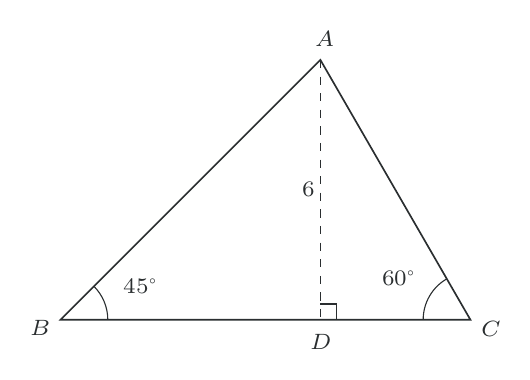
\begin{tikzpicture}[line width=0.6pt,ink,every node/.style={font=\footnotesize,inner sep=1pt}]
\draw[] (0.000mm,33.000mm) -- (-33.000mm,0.000mm) -- (19.053mm,0.000mm) -- cycle;
\draw[dashed] (0.000mm,33.000mm) -- (0.000mm,0.000mm);
\draw[line width=0.4pt] (0.000mm,2.000mm) -- (2.000mm,2.000mm) -- (2.000mm,0.000mm);
\draw[line width=0.4pt] (-27.000mm,0.000mm) arc[start angle=0.000,end angle=45.000,radius=6.000mm];
\node at (-22.837mm,4.210mm) {$45^\circ$};
\draw[line width=0.4pt] (16.053mm,5.196mm) arc[start angle=120.000,end angle=180.000,radius=6.000mm];
\node at (9.959mm,5.250mm) {$60^\circ$};
\node at (0.579mm,35.739mm) {$A$};
\node at (-35.610mm,-1.013mm) {$B$};
\node at (21.592mm,-1.179mm) {$C$};
\node at (0.000mm,-2.800mm) {$D$};
\node[left=0.5pt] at (0.000mm,16.500mm) {$6$};
\end{tikzpicture}}}{$6+6\sqrt3$}{$6+3\sqrt3$}{$6\sqrt3$}{$6+2\sqrt3$}
\satg{5}{A right triangle has an acute angle $\theta$ with $\tan\theta=\dfrac{24}7$. The hypotenuse of the triangle is $50$. What is the area of the triangle?}
\satq{6}{An equilateral triangle has height $15$. What is its area?}{$\dfrac{225\sqrt3}{4}$}{$75\sqrt3$}{$225$}{$150\sqrt3$}
\satq{7}{In right triangle $XYZ$, the right angle is at $Y$ and $\cos Z=\dfrac7{25}$. What is the value of $\tan X$?}{$\dfrac{24}7$}{$\dfrac{25}{24}$}{$\dfrac7{24}$}{$\dfrac7{25}$}
\satq{8}{A rectangle has a diagonal of length $39$. The diagonal makes an angle $\theta$ with a shorter side, where $\tan\theta=\dfrac{12}5$. What is the area of the rectangle?}{$540$}{$468$}{$270$}{$195$}
}
\end{textblock*}
\begin{textblock*}{\COLW}(\RCOL,32mm)
{\fontsize{10}{12.5}\selectfont
\setkicker{Set 2 (cont.)}{Right triangles and trig}
\satq{9}{The altitude to the hypotenuse of an isosceles right triangle is $8\sqrt2$. What is the area of the triangle?}{$64$}{$128$}{$128\sqrt2$}{$256$}
\satq{10}{In the figure, triangle $ABC$ has a right angle at $B$, and $\overline{BD}\perp\overline{AC}$. If $\sin\angle C=\dfrac5{13}$, what is $\cos\angle ABD$?\figbox{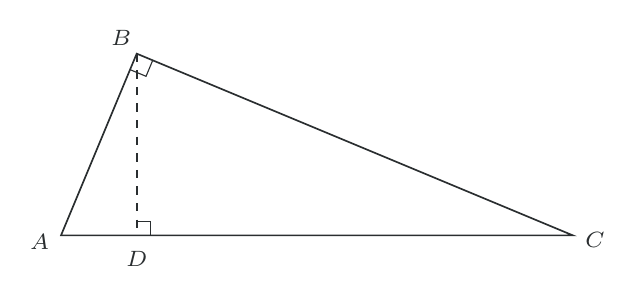
\begin{tikzpicture}[line width=0.6pt,ink,every node/.style={font=\footnotesize,inner sep=1pt}]
\draw[] (0.000mm,0.000mm) -- (9.615mm,23.077mm) -- (65.000mm,0.000mm) -- cycle;
\draw[dashed] (9.615mm,23.077mm) -- (9.615mm,0.000mm);
\draw[line width=0.4pt] (8.769mm,21.046mm) -- (10.800mm,20.200mm) -- (11.646mm,22.231mm);
\draw[line width=0.4pt] (9.615mm,1.800mm) -- (11.415mm,1.800mm) -- (11.415mm,0.000mm);
\node at (-2.675mm,-0.827mm) {$A$};
\node at (7.644mm,25.065mm) {$B$};
\node at (67.750mm,-0.527mm) {$C$};
\node at (9.615mm,-3.000mm) {$D$};
\end{tikzpicture}}}{$\dfrac{12}5$}{$\dfrac{13}{12}$}{$\dfrac{12}{13}$}{$\dfrac5{13}$}
\satg{11}{In right triangle $ABC$, the right angle is at $C$, $\tan A=\dfrac34$, $BC=x+3$ and $AC=2x-2$. What is the length of $\overline{AB}$?}
\satq{12}{The side lengths of a right triangle are $x$, $x+7$ and $x+8$. What is the perimeter of the triangle?}{$13$}{$17$}{$26$}{$30$}
\satg{13}{In right triangle $ABC$, the right angle is at $C$ and $2\sin A=3\cos A$. The area of the triangle is $48$. What is the length of $\overline{BC}$?}
\satq{14}{The perimeter of a $30^\circ$-$60^\circ$-$90^\circ$ triangle is $36+12\sqrt3$. What is the area of the triangle?}{$72\sqrt3$}{$36\sqrt3$}{$144$}{$144\sqrt3$}
}
\end{textblock*}
\clearpage
\topicheader{9}{Hard Triangles \& Chained Geometry}
\pagefooter{3}
\colrule{32}{238}
\mbox{}%
\begin{textblock*}{\COLW}(\LCOL,32mm)
{\fontsize{10}{12.5}\selectfont
\setkicker{Set 3}{Similar triangles, angle chasing and triangle facts.}
\satq{1}{In the figure, point $D$ lies on $\overline{AB}$ and point $E$ lies on $\overline{AC}$, with $\overline{DE}\parallel\overline{BC}$. If $AD=9$, $DB=6$ and $DE=12$, what is the length of $\overline{BC}$?\figbox{\begin{tikzpicture}[line width=0.6pt,ink,every node/.style={font=\footnotesize,inner sep=1pt}]
\draw[] (30.240mm,44.739mm) -- (0.000mm,0.000mm) -- (72.000mm,0.000mm) -- cycle;
\draw[] (12.096mm,17.895mm) -- (55.296mm,17.895mm);
\fill (12.096mm,17.895mm) circle (0.55mm);
\fill (55.296mm,17.895mm) circle (0.55mm);
\node at (29.882mm,47.516mm) {$A$};
\node at (-2.565mm,-1.122mm) {$B$};
\node at (74.606mm,-1.025mm) {$C$};
\node[left=1pt] at (12.096mm,17.895mm) {$D$};
\node[right=1pt] at (55.296mm,17.895mm) {$E$};
\node at (19.180mm,32.661mm) {$9$};
\node at (4.060mm,10.292mm) {$6$};
\node[below=0.5pt] at (33.696mm,17.895mm) {$12$};
\end{tikzpicture}}}{$8$}{$18$}{$20$}{$30$}
\satq{2}{In the figure, lines $m$ and $n$ are parallel and are cut by transversal $t$. What is the value of $x$?\figbox{\begin{tikzpicture}[line width=0.6pt,ink,every node/.style={font=\footnotesize,inner sep=1pt}]
\draw[] (-25.000mm,0.000mm) -- (37.000mm,0.000mm);
\draw[] (-9.378mm,-26.000mm) -- (52.622mm,-26.000mm);
\draw[] (-4.635mm,7.715mm) -- (20.258mm,-33.715mm);
\node[right] at (37.000mm,0.000mm) {$m$};
\node[right] at (52.622mm,-26.000mm) {$n$};
\node[above left] at (-4.635mm,7.715mm) {$t$};
\draw[line width=0.4pt] (3.605mm,-6.000mm) arc[start angle=-59.000,end angle=0.000,radius=7.000mm];
\node at (17.000mm,-6.400mm) {$(3x+5)^\circ$};
\draw[line width=0.4pt] (22.622mm,-26.000mm) arc[start angle=0.000,end angle=121.000,radius=7.000mm];
\node at (32.622mm,-15.500mm) {$(7x-5)^\circ$};
\draw[line width=0.4pt] (-22.200mm,1.100mm) -- (-21.000mm,0.000mm) -- (-22.200mm,-1.100mm);
\draw[line width=0.4pt] (-6.578mm,-24.900mm) -- (-5.378mm,-26.000mm) -- (-6.578mm,-27.100mm);
\end{tikzpicture}}}{$36$}{$18$}{$9$}{$2.5$}
}
\end{textblock*}
\begin{textblock*}{\COLW}(\RCOL,32mm)
{\fontsize{10}{12.5}\selectfont
\setkicker{Set 3 (cont.)}{Similar triangles and angles}
\satg{3}{In the figure, $\angle ABC$ is a right angle, $\overline{BD}\perp\overline{AC}$, $AD=4$ and $DC=9$. What is the area of triangle $ABC$?\figbox{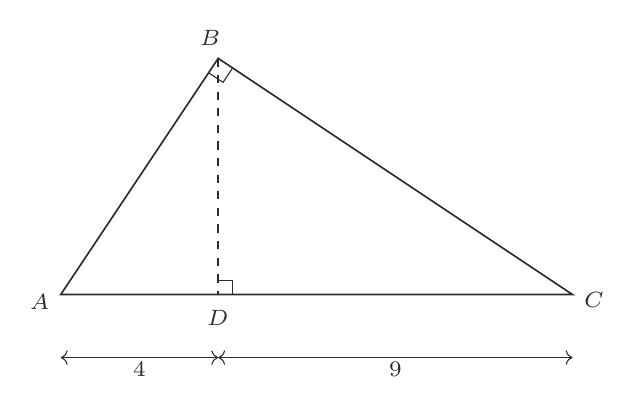
\begin{tikzpicture}[line width=0.6pt,ink,every node/.style={font=\footnotesize,inner sep=1pt}]
\draw[] (0.000mm,0.000mm) -- (20.000mm,30.000mm) -- (65.000mm,0.000mm) -- cycle;
\draw[dashed] (20.000mm,30.000mm) -- (20.000mm,0.000mm);
\draw[line width=0.4pt] (18.780mm,28.169mm) -- (20.610mm,26.949mm) -- (21.831mm,28.780mm);
\draw[line width=0.4pt] (20.000mm,1.800mm) -- (21.800mm,1.800mm) -- (21.800mm,0.000mm);
\node at (-2.640mm,-0.932mm) {$A$};
\node at (18.923mm,32.585mm) {$B$};
\node at (67.701mm,-0.737mm) {$C$};
\node at (20.000mm,-3.000mm) {$D$};
\draw[<->,line width=0.4pt] (0.000mm,-8.000mm) -- (20.000mm,-8.000mm);
\draw[<->,line width=0.4pt] (20.000mm,-8.000mm) -- (65.000mm,-8.000mm);
\node[below=0.3pt] at (10.000mm,-8.000mm) {$4$};
\node[below=0.3pt] at (42.500mm,-8.000mm) {$9$};
\end{tikzpicture}}}
\satq{4}{In triangle $ABC$, points $M$ and $N$ are the midpoints of $\overline{AB}$ and $\overline{AC}$. If $MN=2x+3$ and $BC=5x-3$, what is the length of $\overline{BC}$?}{$7$}{$9$}{$21$}{$42$}
\satg{5}{In the figure, $AB=AC$. The measure of $\angle A$ is $(3x-6)^\circ$ and the measure of exterior angle $\angle ACD$ is $(7x+10)^\circ$. What is the value of $x$?\figbox{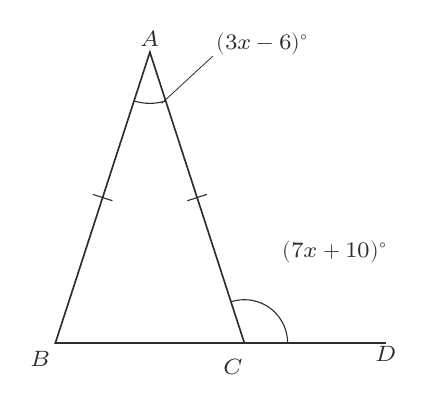
\begin{tikzpicture}[line width=0.6pt,ink,every node/.style={font=\footnotesize,inner sep=1pt}]
\draw[] (12.000mm,36.932mm) -- (0.000mm,0.000mm) -- (24.000mm,0.000mm) -- cycle;
\draw[] (24.000mm,0.000mm) -- (42.000mm,0.000mm);
\draw[line width=0.4pt] (7.236mm,18.064mm) -- (4.764mm,18.868mm);
\draw[line width=0.4pt] (19.236mm,18.868mm) -- (16.764mm,18.064mm);
\node at (-1.954mm,-2.005mm) {$B$};
\node at (22.500mm,-3.000mm) {$C$};
\node[below] at (42.000mm,0.000mm) {$D$};
\node[above=0.3mm] at (12.000mm,36.932mm) {$A$};
\draw[line width=0.4pt] (9.991mm,30.750mm) arc[start angle=-108.000,end angle=-72.000,radius=6.500mm];
\draw[line width=0.3pt] (20.000mm,36.432mm) -- (13.500mm,30.432mm);
\node[right=0pt] at (20.000mm,37.932mm) {$(3x-6)^\circ$};
\draw[line width=0.4pt] (29.500mm,0.000mm) arc[start angle=0.000,end angle=108.000,radius=5.500mm];
\node at (35.500mm,11.500mm) {$(7x+10)^\circ$};
\end{tikzpicture}}}
\satg{6}{The side lengths of a triangle are $9$, $14$ and $3x$, where $x$ is a positive integer. How many possible values of $x$ are there?}
}
\end{textblock*}
\clearpage
\topicheader{9}{Hard Triangles \& Chained Geometry}
\pagefooter{4}
\colrule{32}{238}
\mbox{}%
\begin{textblock*}{\COLW}(\LCOL,32mm)
{\fontsize{10}{12.5}\selectfont
\setkicker{Set 3 (cont.)}{Similar triangles and angles}
\satq{7}{In the figure, convex pentagon $ABCDE$ has $\overline{AB}\parallel\overline{ED}$. The angles are $\angle B=(2x+30)^\circ$, $\angle C=(3x-10)^\circ$ and $\angle D=(x+40)^\circ$. What is the measure of $\angle C$?\figbox{\begin{tikzpicture}[line width=0.6pt,ink,every node/.style={font=\footnotesize,inner sep=1pt}]
\draw[] (0.000mm,0.000mm) -- (31.200mm,0.000mm) -- (46.241mm,17.925mm) -- (46.241mm,36.125mm) -- (-6.370mm,36.125mm) -- cycle;
\draw[line width=0.4pt] (14.400mm,1.100mm) -- (15.600mm,0.000mm) -- (14.400mm,-1.100mm);
\draw[line width=0.4pt] (18.736mm,37.225mm) -- (19.936mm,36.125mm) -- (18.736mm,35.025mm);
\node at (-2.379mm,-1.828mm) {$A$};
\node at (32.383mm,-2.757mm) {$B$};
\node at (49.241mm,17.911mm) {$C$};
\node at (48.591mm,37.991mm) {$D$};
\node at (-8.935mm,37.681mm) {$E$};
\draw[line width=0.4pt] (33.771mm,3.064mm) arc[start angle=50.000,end angle=180.000,radius=4.000mm];
\node at (34.946mm,-8.730mm) {$(2x+30)^\circ$};
\draw[line width=0.4pt] (46.241mm,21.925mm) arc[start angle=-270.000,end angle=-130.000,radius=4.000mm];
\node at (56.741mm,17.875mm) {$(3x-10)^\circ$};
\draw[line width=0.4pt] (46.241mm,33.725mm) -- (43.841mm,33.725mm) -- (43.841mm,36.125mm);
\node at (53.681mm,42.034mm) {$(x+40)^\circ$};
\end{tikzpicture}}}{$140^\circ$}{$130^\circ$}{$90^\circ$}{$50^\circ$}
\satq{8}{In triangle $ABC$, point $D$ is on $\overline{AB}$ and point $E$ is on $\overline{AC}$ with $\overline{DE}\parallel\overline{BC}$ and $AD:DB=2:3$. The area of triangle $ABC$ is $100$. What is the area of quadrilateral $DBCE$?}{$16$}{$40$}{$60$}{$84$}
\satq{9}{In triangle $ABC$, medians $\overline{AD}$ and $\overline{BE}$ meet at $G$. If $AG=4x+2$ and $GD=x+7$, what is the length of $\overline{AD}$?}{$13$}{$26$}{$39$}{$52$}
\satqw{10}{A triangle has side lengths $9$, $12$ and $14$. Which statement about its largest angle is true?}{It is less than $90^\circ$.}{It measures exactly $90^\circ$.}{It is greater than $90^\circ$.}{Its measure cannot be found from the side lengths.}
}
\end{textblock*}
\begin{textblock*}{\COLW}(\RCOL,32mm)
{\fontsize{10}{12.5}\selectfont
\setkicker{Set 3 (cont.)}{Similar triangles and angles}
\satq{11}{In the figure, segments $\overline{AD}$ and $\overline{BC}$ intersect at $E$, and $\overline{AB}\parallel\overline{DC}$. If $AE=12$, $ED=18$ and $BE=10$, what is the length of $\overline{BC}$?\figbox{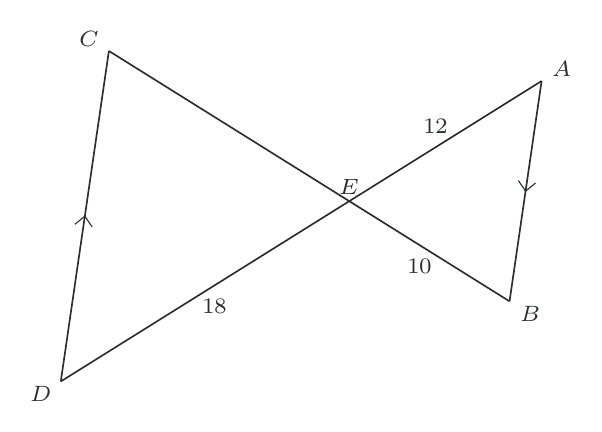
\begin{tikzpicture}[line width=0.6pt,ink,every node/.style={font=\footnotesize,inner sep=1pt}]
\draw[] (24.424mm,15.262mm) -- (-36.636mm,-22.893mm);
\draw[] (20.353mm,-12.718mm) -- (-30.530mm,19.077mm);
\draw[] (24.424mm,15.262mm) -- (20.353mm,-12.718mm);
\draw[] (-36.636mm,-22.893mm) -- (-30.530mm,19.077mm);
\draw[line width=0.4pt] (23.650mm,2.301mm) -- (22.388mm,1.272mm) -- (21.473mm,2.618mm);
\draw[line width=0.4pt] (-34.844mm,-2.937mm) -- (-33.583mm,-1.908mm) -- (-32.667mm,-3.254mm);
\node at (26.968mm,16.851mm) {$A$};
\node at (22.897mm,-14.308mm) {$B$};
\node at (-33.074mm,20.667mm) {$C$};
\node at (-39.180mm,-24.482mm) {$D$};
\node[above=1pt] at (0.000mm,0.000mm) {$E$};
\node at (10.993mm,9.581mm) {$12$};
\node at (-17.099mm,-13.397mm) {$18$};
\node at (8.958mm,-8.310mm) {$10$};
\end{tikzpicture}}}{$15$}{$\dfrac{50}{3}$}{$22$}{$25$}
\satq{12}{Each interior angle of a regular polygon measures $(4x+10)^\circ$ and each exterior angle measures $(x-5)^\circ$. How many sides does the polygon have?}{$6$}{$12$}{$30$}{$35$}
\satg{13}{Two similar triangles have perimeters $24$ and $40$. The larger triangle has area $250$. What is the area of the smaller triangle?}
}
\end{textblock*}
\clearpage
\topicheader{9}{Hard Triangles \& Chained Geometry}
\pagefooter{5}
\colrule{32}{238}
\mbox{}%
\begin{textblock*}{\COLW}(\LCOL,32mm)
{\fontsize{10}{12.5}\selectfont
\setkicker{Set 3 (cont.)}{Similar triangles and angles}
\satq{14}{In the figure, triangle $ABC$ has $AB=AC$, and point $D$ lies on $\overline{AC}$ so that $AD=BD=BC$. What is the measure of $\angle ABC$?\figbox{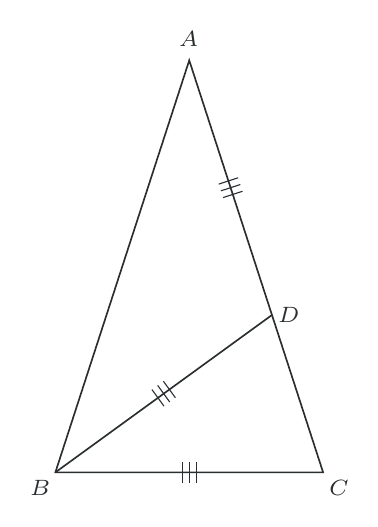
\begin{tikzpicture}[line width=0.6pt,ink,every node/.style={font=\footnotesize,inner sep=1pt}]
\draw[] (17.000mm,52.321mm) -- (0.000mm,0.000mm) -- (34.000mm,0.000mm) -- cycle;
\draw[] (0.000mm,0.000mm) -- (27.507mm,19.985mm);
\draw[line width=0.4pt] (23.212mm,37.410mm) -- (20.739mm,36.607mm);
\draw[line width=0.4pt] (23.490mm,36.554mm) -- (21.017mm,35.751mm);
\draw[line width=0.4pt] (23.768mm,35.698mm) -- (21.295mm,34.895mm);
\draw[line width=0.4pt] (12.261mm,10.515mm) -- (13.789mm,8.412mm);
\draw[line width=0.4pt] (12.989mm,11.044mm) -- (14.517mm,8.941mm);
\draw[line width=0.4pt] (13.717mm,11.573mm) -- (15.246mm,9.470mm);
\draw[line width=0.4pt] (16.100mm,1.300mm) -- (16.100mm,-1.300mm);
\draw[line width=0.4pt] (17.000mm,1.300mm) -- (17.000mm,-1.300mm);
\draw[line width=0.4pt] (17.900mm,1.300mm) -- (17.900mm,-1.300mm);
\node at (17.000mm,55.121mm) {$A$};
\node at (-1.954mm,-2.005mm) {$B$};
\node at (35.954mm,-2.005mm) {$C$};
\node[right=1pt] at (27.507mm,19.985mm) {$D$};
\end{tikzpicture}}}{$36^\circ$}{$60^\circ$}{$72^\circ$}{$108^\circ$}
\vspace{3mm}
\setkicker{Set 4}{Chained geometry: coordinates, composite figures, word problems.}
\satq{1}{In the figure, $AB=13$, $BC=20$ and $AC=21$. What is the area of triangle $ABC$?\figbox{\begin{tikzpicture}[line width=0.6pt,ink,every node/.style={font=\footnotesize,inner sep=1pt}]
\draw[] (0.000mm,0.000mm) -- (17.000mm,40.800mm) -- (71.400mm,0.000mm) -- cycle;
\node at (-2.542mm,-1.173mm) {$A$};
\node at (15.833mm,43.345mm) {$B$};
\node at (74.063mm,-0.864mm) {$C$};
\node at (6.100mm,21.400mm) {$13$};
\node at (45.760mm,22.480mm) {$20$};
\node at (35.700mm,-2.600mm) {$21$};
\end{tikzpicture}}}{$126$}{$130$}{$136.5$}{$210$}
}
\end{textblock*}
\begin{textblock*}{\COLW}(\RCOL,32mm)
{\fontsize{10}{12.5}\selectfont
\setkicker{Set 4 (cont.)}{Chained geometry}
\satq{2}{A tower stands on level ground. Points $A$ and $B$ are on the ground in line with the base $O$ of the tower, with $A$ between $B$ and $O$ and $AB=40$ meters. The angle of elevation of the top $T$ of the tower is $45^\circ$ from $A$ and $30^\circ$ from $B$. What is the height of the tower, in meters?\figbox{\begin{tikzpicture}[line width=0.6pt,ink,every node/.style={font=\footnotesize,inner sep=1pt}]
\draw[] (-77.820mm,0.000mm) -- (7.000mm,0.000mm);
\draw[] (0.000mm,0.000mm) -- (0.000mm,42.620mm);
\draw[] (-73.820mm,0.000mm) -- (0.000mm,42.620mm);
\draw[] (-42.620mm,0.000mm) -- (0.000mm,42.620mm);
\draw[line width=0.4pt] (0.000mm,2.200mm) -- (-2.200mm,2.200mm) -- (-2.200mm,0.000mm);
\node[above] at (0.000mm,42.620mm) {$T$};
\node[below] at (-73.820mm,0.000mm) {$B$};
\node[below] at (-42.620mm,0.000mm) {$A$};
\node[below] at (0.000mm,0.000mm) {$O$};
\fill (-42.620mm,0.000mm) circle (0.55mm);
\fill (-73.820mm,0.000mm) circle (0.55mm);
\draw[line width=0.4pt] (-64.820mm,0.000mm) arc[start angle=0.000,end angle=30.000,radius=9.000mm];
\node at (-57.820mm,2.000mm) {$30^\circ$};
\draw[line width=0.4pt] (-36.620mm,0.000mm) arc[start angle=0.000,end angle=45.000,radius=6.000mm];
\node at (-31.620mm,4.000mm) {$45^\circ$};
\draw[<->,line width=0.4pt] (-73.820mm,-7.300mm) -- (-42.620mm,-7.300mm);
\node[below] at (-58.220mm,-7.000mm) {$40$ m};
\end{tikzpicture}}}{$40\sqrt3$}{$20(\sqrt3+1)$}{$20\sqrt3$}{$40(\sqrt3-1)$}
\satq{3}{A $25$-foot ladder leans against a vertical wall with its top $24$ feet above the ground. The foot of the ladder is pulled away from the wall until the top of the ladder is $20$ feet above the ground. How many feet did the foot of the ladder move?}{$22$}{$15$}{$8$}{$4$}
\satg{4}{In the $xy$-plane, $P=(-2,1)$ and $R=(7,-2)$. Point $Q$ has coordinates $(4,k)$, and $\angle PQR$ is a right angle. What is the sum of all possible values of $k$?\figbox{\begin{tikzpicture}[line width=0.6pt,ink,every node/.style={font=\footnotesize,inner sep=1pt}]
\draw[->,line width=0.4pt] (-15.840mm,0.000mm) -- (38.720mm,0.000mm);
\draw[->,line width=0.4pt] (0.000mm,-29.040mm) -- (0.000mm,20.240mm);
\node[right] at (38.720mm,0.000mm) {$x$};
\node[above] at (0.000mm,20.240mm) {$y$};
\draw[line width=0.3pt] (-13.200mm,-0.900mm) -- (-13.200mm,0.900mm);
\draw[line width=0.3pt] (-8.800mm,-0.900mm) -- (-8.800mm,0.900mm);
\draw[line width=0.3pt] (-4.400mm,-0.900mm) -- (-4.400mm,0.900mm);
\draw[line width=0.3pt] (4.400mm,-0.900mm) -- (4.400mm,0.900mm);
\draw[line width=0.3pt] (8.800mm,-0.900mm) -- (8.800mm,0.900mm);
\draw[line width=0.3pt] (13.200mm,-0.900mm) -- (13.200mm,0.900mm);
\draw[line width=0.3pt] (17.600mm,-0.900mm) -- (17.600mm,0.900mm);
\draw[line width=0.3pt] (22.000mm,-0.900mm) -- (22.000mm,0.900mm);
\draw[line width=0.3pt] (26.400mm,-0.900mm) -- (26.400mm,0.900mm);
\draw[line width=0.3pt] (30.800mm,-0.900mm) -- (30.800mm,0.900mm);
\draw[line width=0.3pt] (35.200mm,-0.900mm) -- (35.200mm,0.900mm);
\draw[line width=0.3pt] (-0.900mm,-26.400mm) -- (0.900mm,-26.400mm);
\draw[line width=0.3pt] (-0.900mm,-22.000mm) -- (0.900mm,-22.000mm);
\draw[line width=0.3pt] (-0.900mm,-17.600mm) -- (0.900mm,-17.600mm);
\draw[line width=0.3pt] (-0.900mm,-13.200mm) -- (0.900mm,-13.200mm);
\draw[line width=0.3pt] (-0.900mm,-8.800mm) -- (0.900mm,-8.800mm);
\draw[line width=0.3pt] (-0.900mm,-4.400mm) -- (0.900mm,-4.400mm);
\draw[line width=0.3pt] (-0.900mm,4.400mm) -- (0.900mm,4.400mm);
\draw[line width=0.3pt] (-0.900mm,8.800mm) -- (0.900mm,8.800mm);
\draw[line width=0.3pt] (-0.900mm,13.200mm) -- (0.900mm,13.200mm);
\draw[line width=0.3pt] (-0.900mm,17.600mm) -- (0.900mm,17.600mm);
\draw[dashed] (17.600mm,-27.280mm) -- (17.600mm,18.480mm);
\node[above right] at (17.600mm,13.200mm) {$x=4$};
\draw[] (-8.800mm,4.400mm) -- (30.800mm,-8.800mm);
\fill (-8.800mm,4.400mm) circle (0.55mm);
\node[above left] at (-8.800mm,4.400mm) {$P({-}2,1)$};
\fill (30.800mm,-8.800mm) circle (0.55mm);
\node[below right] at (30.800mm,-8.800mm) {$R(7,{-}2)$};
\end{tikzpicture}}}
}
\end{textblock*}
\clearpage
\topicheader{9}{Hard Triangles \& Chained Geometry}
\pagefooter{6}
\colrule{32}{238}
\mbox{}%
\begin{textblock*}{\COLW}(\LCOL,32mm)
{\fontsize{10}{12.5}\selectfont
\setkicker{Set 4 (cont.)}{Chained geometry}
\satg{5}{In the $xy$-plane, $A=(1,1)$, $B=(13,1)$ and $C=(7,k)$, where $k>0$. The area of triangle $ABC$ is $48$. What is the perimeter of triangle $ABC$?}
\satq{6}{The figure is a rectangle topped by an isosceles triangle. The rectangle measures $12$ by $6$, and each of the two equal sides of the triangle is $10$. What is the area of the whole figure?\figbox{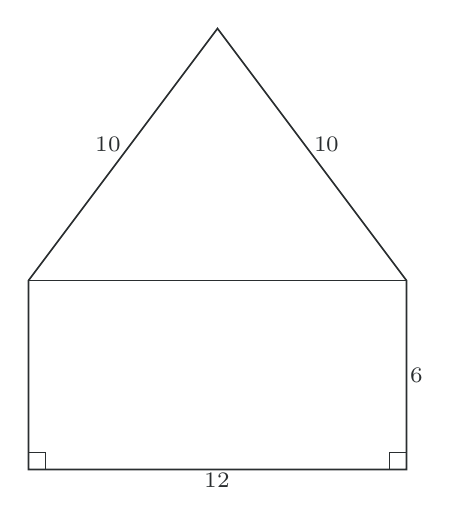
\begin{tikzpicture}[line width=0.6pt,ink,every node/.style={font=\footnotesize,inner sep=1pt}]
\draw[] (0.000mm,0.000mm) -- (48.000mm,0.000mm) -- (48.000mm,24.000mm) -- (24.000mm,56.000mm) -- (0.000mm,24.000mm) -- cycle;
\draw[] (0.000mm,24.000mm) -- (48.000mm,24.000mm);
\draw[line width=0.4pt] (2.200mm,0.000mm) -- (2.200mm,2.200mm) -- (0.000mm,2.200mm);
\draw[line width=0.4pt] (48.000mm,2.200mm) -- (45.800mm,2.200mm) -- (45.800mm,0.000mm);
\node[below] at (24.000mm,0.000mm) {$12$};
\node[right] at (48.000mm,12.000mm) {$6$};
\node[above left=-0.5pt] at (12.000mm,40.000mm) {$10$};
\node[above right=-0.5pt] at (36.000mm,40.000mm) {$10$};
\end{tikzpicture}}}{$48$}{$120$}{$132$}{$168$}
\satq{7}{A vertical pole stands on level ground. Two straight cables run from the top of the pole to points $A$ and $B$ on the ground on opposite sides of the pole. The cables are $17$ meters and $10$ meters long, and $A$ and $B$ are $21$ meters apart. How tall is the pole, in meters?}{$6$}{$9$}{$15$}{$8$}
}
\end{textblock*}
\begin{textblock*}{\COLW}(\RCOL,32mm)
{\fontsize{10}{12.5}\selectfont
\setkicker{Set 4 (cont.)}{Chained geometry}
\satg{8}{In the figure, $\angle ABC$ and $\angle ACD$ are right angles, $AB=9$, $\tan\angle BAC=\dfrac43$ and $\sin\angle CAD=\dfrac45$. What is the perimeter of quadrilateral $ABCD$?\figbox{\begin{tikzpicture}[line width=0.6pt,ink,every node/.style={font=\footnotesize,inner sep=1pt}]
\draw[] (0.000mm,27.000mm) -- (0.000mm,0.000mm) -- (36.000mm,0.000mm) -- (72.000mm,48.000mm) -- cycle;
\draw[] (0.000mm,27.000mm) -- (36.000mm,0.000mm);
\draw[line width=0.4pt] (0.000mm,2.200mm) -- (2.200mm,2.200mm) -- (2.200mm,0.000mm);
\draw[line width=0.4pt] (34.240mm,1.320mm) -- (35.560mm,3.080mm) -- (37.320mm,1.760mm);
\node at (-2.869mm,27.877mm) {$A$};
\node at (-2.464mm,-1.711mm) {$B$};
\node at (37.298mm,-2.705mm) {$C$};
\node at (74.515mm,49.635mm) {$D$};
\node[left] at (0.000mm,13.500mm) {$9$};
\end{tikzpicture}}}
\satq{9}{A lamp is fixed to the top of a vertical post on level ground. A person $1.5$ m tall stands $6$ m from the post and casts a shadow $2$ m long (the shadow points away from the post). The person then walks directly away from the post until the shadow is $4$ m long. How many meters did the person walk?}{$2$}{$4$}{$6$}{$12$}
\satq{10}{Point $A=(2,-1)$ and point $B=(8,7)$. Which of the following points lies on the perpendicular bisector of $\overline{AB}$?}{$(9,0)$}{$(9,6)$}{$(8,-1)$}{$(6,-4)$}
\satq{11}{A rectangle has a diagonal of length $25$, and its two side lengths differ by $5$. What is the perimeter of the rectangle?}{$100$}{$70$}{$50$}{$35$}
\satq{12}{An isosceles triangle has a base of $16$ and a perimeter of $36$. What is its area?}{$96$}{$80$}{$64$}{$48$}
}
\end{textblock*}
\clearpage
\topicheader{9}{Hard Triangles \& Chained Geometry}
\pagefooter{7}
\colrule{32}{238}
\mbox{}%
\begin{textblock*}{\COLW}(\LCOL,32mm)
{\fontsize{10}{12.5}\selectfont
\setkicker{Set 4 (cont.)}{Chained geometry}
\satg{13}{In the figure, a square is placed inside right triangle $ABC$ with one vertex at the right-angle vertex $C$ and the opposite vertex on the hypotenuse $\overline{AB}$. The legs are $CB=12$ and $CA=6$. What is the side length of the square?\figbox{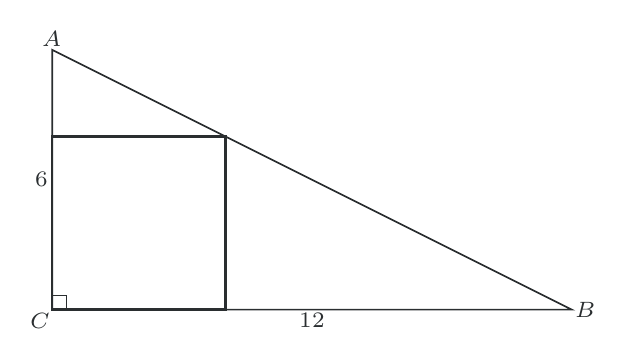
\begin{tikzpicture}[line width=0.6pt,ink,every node/.style={font=\footnotesize,inner sep=1pt}]
\draw[] (0.000mm,0.000mm) -- (66.000mm,0.000mm) -- (0.000mm,33.000mm) -- cycle;
\draw[line width=0.9pt] (0.000mm,0.000mm) -- (22.000mm,0.000mm) -- (22.000mm,22.000mm) -- (0.000mm,22.000mm) -- cycle;
\draw[line width=0.4pt] (1.800mm,0.000mm) -- (1.800mm,1.800mm) -- (0.000mm,1.800mm);
\node[below] at (33.000mm,0.000mm) {$12$};
\node[left] at (0.000mm,16.500mm) {$6$};
\node[below left] at (0.000mm,0.000mm) {$C$};
\node[right] at (66.000mm,0.000mm) {$B$};
\node[above] at (0.000mm,33.000mm) {$A$};
\end{tikzpicture}}}
\satq{14}{A rectangular box measures $6$ by $8$ by $24$. What is the length of the longest segment that can be drawn between two corners of the box?}{$676$}{$38$}{$26$}{$10$}
\vspace{3mm}
\setkicker{Set 5}{Summit: the hardest mixed problems.}
\satq{1}{In right triangle $ABC$, the right angle is at $C$, and $\overline{CH}$ is the altitude to hypotenuse $\overline{AB}$ with $H$ on $\overline{AB}$. If $CH=12$, $AH=x$ and $HB=x+7$, what is the perimeter of triangle $ABC$?}{$25$}{$37$}{$49$}{$60$}
\satg{2}{In right triangle $ABC$, the right angle is at $C$. The area of the triangle is $6$, and $\tan A+\tan B=\dfrac{25}{12}$. What is the length of the hypotenuse?}
\satq{3}{In trapezoid $ABCD$, $\overline{AB}\parallel\overline{CD}$, $AB=8$ and $CD=12$. The diagonals meet at $E$, and the area of triangle $CDE$ is $90$. What is the area of triangle $ABE$?}{$40$}{$50$}{$60$}{$135$}
}
\end{textblock*}
\begin{textblock*}{\COLW}(\RCOL,32mm)
{\fontsize{10}{12.5}\selectfont
\setkicker{Set 5 (cont.)}{Summit}
\satg{4}{Two sides of a triangle measure $7$ and $8$, and the third side has integer length $x$. For how many values of $x$ is the triangle obtuse?}
\satq{5}{A circle is inscribed in a right triangle with legs $9$ and $12$, touching all three sides. What is the area of the circle?}{$\dfrac{9\pi}{4}$}{$9\pi$}{$36\pi$}{$\dfrac{225\pi}{4}$}
\satq{6}{In the $xy$-plane, point $P$ lies on the line $y=\dfrac34x$ in the first quadrant, and $P$ is $20$ units from the origin. What is the sum of the coordinates of $P$?}{$7$}{$20$}{$28$}{$35$}
\satq{7}{Two vertical poles of heights $12$ m and $20$ m stand $15$ m apart on level ground. A cable runs from the top of each pole to the base of the other, and the cables cross at point $X$. How many meters above the ground is $X$?\figbox{\begin{tikzpicture}[line width=0.6pt,ink,every node/.style={font=\footnotesize,inner sep=1pt}]
\draw[] (-5.000mm,0.000mm) -- (50.000mm,0.000mm);
\draw[] (0.000mm,0.000mm) -- (0.000mm,36.000mm);
\draw[] (45.000mm,0.000mm) -- (45.000mm,60.000mm);
\draw[line width=0.5pt] (0.000mm,0.000mm) -- (45.000mm,60.000mm);
\draw[line width=0.5pt] (45.000mm,0.000mm) -- (0.000mm,36.000mm);
\node[left] at (0.000mm,18.000mm) {$12$};
\node[right] at (45.000mm,30.000mm) {$20$};
\node[below] at (22.500mm,0.000mm) {$15$};
\fill (0.000mm,36.000mm) circle (0.55mm);
\fill (45.000mm,60.000mm) circle (0.55mm);
\end{tikzpicture}}}{$7.5$}{$16$}{$32$}{$240$}
\satg{8}{The side lengths of a right triangle form an arithmetic sequence, and the area of the triangle is $54$. What is the perimeter of the triangle?}
}
\end{textblock*}
\clearpage
\topicheader{9}{Hard Triangles \& Chained Geometry}
\pagefooter{8}
\colrule{32}{238}
\mbox{}%
\begin{textblock*}{\COLW}(\LCOL,32mm)
{\fontsize{10}{12.5}\selectfont
\setkicker{Set 5 (cont.)}{Summit}
\satq{9}{A regular hexagon $ABCDEF$ has side length $6$. Triangle $ACE$ is formed by joining alternate vertices. What is the area of triangle $ACE$?\figbox{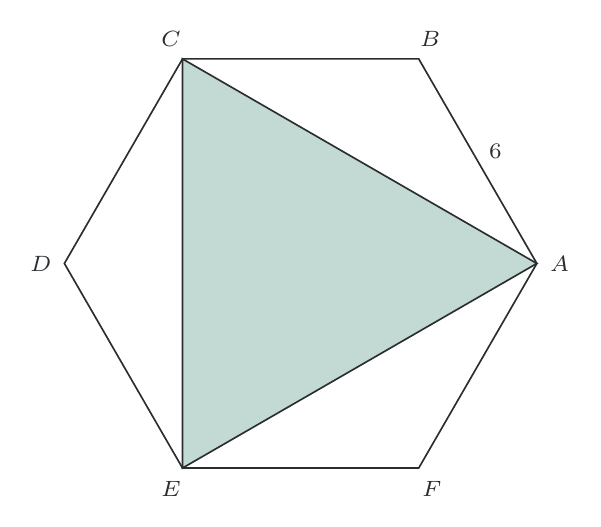
\begin{tikzpicture}[line width=0.6pt,ink,every node/.style={font=\footnotesize,inner sep=1pt}]
\fill[accent!25] (30.000mm,0.000mm) -- (-15.000mm,25.981mm) -- (-15.000mm,-25.981mm) -- cycle;
\draw[] (30.000mm,0.000mm) -- (15.000mm,25.981mm) -- (-15.000mm,25.981mm) -- (-30.000mm,0.000mm) -- (-15.000mm,-25.981mm) -- (15.000mm,-25.981mm) -- cycle;
\draw[] (30.000mm,0.000mm) -- (-15.000mm,25.981mm) -- (-15.000mm,-25.981mm) -- cycle;
\node at (33.000mm,0.000mm) {$A$};
\node at (16.500mm,28.579mm) {$B$};
\node at (-16.500mm,28.579mm) {$C$};
\node at (-33.000mm,0.000mm) {$D$};
\node at (-16.500mm,-28.579mm) {$E$};
\node at (16.500mm,-28.579mm) {$F$};
\node at (24.752mm,14.290mm) {$6$};
\end{tikzpicture}}}{$54\sqrt3$}{$27\sqrt3$}{$18\sqrt3$}{$9\sqrt3$}
\satq{10}{In a regular decagon (a polygon with $10$ equal sides and equal angles) $ABCDEFGHIJ$, what is the measure of $\angle ACD$?}{$162^\circ$}{$144^\circ$}{$126^\circ$}{$18^\circ$}
\satg{11}{Rectangle $ABCD$ has $AB=12$ and $BC=16$. The perpendicular from $A$ to diagonal $\overline{BD}$ meets $\overline{BD}$ at $H$. What is the value of $DH-BH$?}
\satq{12}{From the top of a vertical tower $30$ m tall, the angles of depression of two cars on the level road, in line with the base of the tower and on opposite sides of it, are $45^\circ$ and $30^\circ$. How far apart are the cars, in meters?}{$30\sqrt3-30$}{$30\sqrt3$}{$60$}{$30+30\sqrt3$}
\satq{13}{In parallelogram $ABCD$, $AB=14$, $AD=10$ and $\angle A=60^\circ$. What is the area of the parallelogram?}{$140$}{$70\sqrt3$}{$70$}{$35\sqrt3$}
}
\end{textblock*}
\begin{textblock*}{\COLW}(\RCOL,32mm)
{\fontsize{10}{12.5}\selectfont
\setkicker{Set 5 (cont.)}{Summit}
\satg{14}{An isosceles triangle has two sides of length $25$ and an area of $168$. What is the sum of all possible lengths of the third side?}
\satq{15}{In isosceles trapezoid $ABCD$, $\overline{AB}\parallel\overline{DC}$, $AB=10$, $DC=26$ and $AD=BC=10$. What is the area of the trapezoid?\figbox{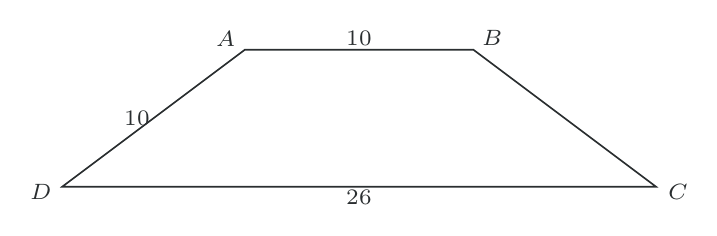
\begin{tikzpicture}[line width=0.6pt,ink,every node/.style={font=\footnotesize,inner sep=1pt}]
\draw[] (0.000mm,0.000mm) -- (75.400mm,0.000mm) -- (52.200mm,17.400mm) -- (23.200mm,17.400mm) -- cycle;
\node at (-2.728mm,-0.630mm) {$D$};
\node at (78.128mm,-0.630mm) {$C$};
\node at (54.601mm,18.841mm) {$B$};
\node at (20.799mm,18.841mm) {$A$};
\node[above] at (37.700mm,17.400mm) {$10$};
\node[below] at (37.700mm,0.000mm) {$26$};
\node[left] at (11.600mm,8.700mm) {$10$};
\end{tikzpicture}}}{$108$}{$156$}{$180$}{$216$}
\satq{16}{In right triangle $ABC$, the right angle is at $B$ and the legs are $AB=9$ and $BC=12$. Point $D$ is on $\overline{AB}$ and point $E$ is on $\overline{BC}$ with $\overline{DE}\parallel\overline{AC}$, and the area of triangle $DBE$ is one-fourth the area of triangle $ABC$. What is the length of $\overline{DE}$?}{$3.75$}{$11.25$}{$30$}{$7.5$}
\satq{17}{Square $ABCD$ has side length $12$. Point $E$ is the midpoint of $\overline{AB}$ and point $F$ is the midpoint of $\overline{BC}$. What is the area of triangle $DEF$?}{$54$}{$36$}{$72$}{$90$}
}
\end{textblock*}
\clearpage
\topicheader{9}{Hard Triangles \& Chained Geometry}
\pagefooter{9}
\colrule{32}{238}
\mbox{}%
\begin{textblock*}{\COLW}(\LCOL,32mm)
{\fontsize{10}{12.5}\selectfont
\setkicker{Set 5 (cont.)}{Summit}
\satq{18}{In the figure, triangle $ABC$ has a right angle at $C$ and $\tan B=\dfrac12$. Point $D$ is on $\overline{BC}$ with $BD=4$ and $DC=6$. What is $\tan\angle ADC$?\figbox{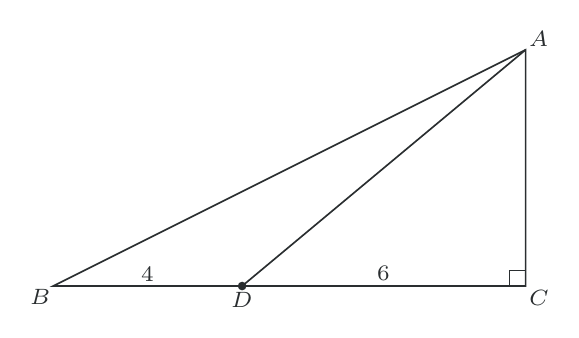
\begin{tikzpicture}[line width=0.6pt,ink,every node/.style={font=\footnotesize,inner sep=1pt}]
\draw[] (60.000mm,30.000mm) -- (0.000mm,0.000mm) -- (60.000mm,0.000mm) -- cycle;
\draw[] (60.000mm,30.000mm) -- (24.000mm,0.000mm);
\fill (24.000mm,0.000mm) circle (0.55mm);
\draw[line width=0.4pt] (60.000mm,2.000mm) -- (58.000mm,2.000mm) -- (58.000mm,0.000mm);
\node[below left] at (0.000mm,0.000mm) {$B$};
\node[below right] at (60.000mm,0.000mm) {$C$};
\node[above right] at (60.000mm,30.000mm) {$A$};
\node[below=1pt] at (24.000mm,0.000mm) {$D$};
\node[above=0.5pt] at (12.000mm,0.000mm) {$4$};
\node[above=0.5pt] at (42.000mm,0.000mm) {$6$};
\end{tikzpicture}}}{$\dfrac12$}{$\dfrac65$}{$\dfrac54$}{$\dfrac56$}
\satg{19}{In the $xy$-plane, point $P$ lies on the $x$-axis and is equally distant from $A=(0,6)$ and $B=(8,2)$. What is the area of triangle $PAB$?}
\satq{20}{Which of the following lists of side lengths forms a right triangle?}{$9,\ 40,\ 41$}{$8,\ 15,\ 16$}{$12,\ 35,\ 36$}{$20,\ 21,\ 28$}
}
\end{textblock*}
\clearpage
\topicheader{9}{Hard Triangles \& Chained Geometry}
\pagefooter{10}
\mbox{}%
\begin{textblock*}{178mm}(16mm,30mm)
{\bfseries\itshape\color{accent}\fontsize{19}{21}\selectfont\centering Answer Key\par}
\end{textblock*}
\begin{textblock*}{178mm}(16mm,41mm)
{\fontsize{9.5}{12}\selectfont\color{black!70}\centering Multiple choice: the letter. Grid-in: the number to enter. Worked solutions follow on the next pages.\par}
\end{textblock*}
\begin{textblock*}{178mm}(16mm,52mm)
{\fontsize{10}{13}\selectfont
\centering
\setlength{\tabcolsep}{2pt}\renewcommand{\arraystretch}{1.3}
{\sffamily\bfseries\color{accent}\fontsize{11}{13}\selectfont Set 1 \ \textmd{\itshape\small Bridge: the core moves}}\\[1.3mm]
\begin{tabular}{|>{\centering\arraybackslash}p{16mm}|>{\centering\arraybackslash}p{16mm}|>{\centering\arraybackslash}p{16mm}|>{\centering\arraybackslash}p{16mm}|>{\centering\arraybackslash}p{16mm}|>{\centering\arraybackslash}p{16mm}|>{\centering\arraybackslash}p{16mm}|>{\centering\arraybackslash}p{16mm}|>{\centering\arraybackslash}p{16mm}|>{\centering\arraybackslash}p{16mm}|}
\hline
\cellcolor{badge!55}\textbf{1} & \cellcolor{badge!55}\textbf{2} & \cellcolor{badge!55}\textbf{3} & \cellcolor{badge!55}\textbf{4} & \cellcolor{badge!55}\textbf{5} & \cellcolor{badge!55}\textbf{6} & \cellcolor{badge!55}\textbf{7} & \cellcolor{badge!55}\textbf{8} & \cellcolor{badge!55}\textbf{9} & \cellcolor{badge!55}\textbf{10}\\
\hline
\textbf{A} & 11 & 37 & \textbf{C} & \textbf{B} & \textbf{C} & \textbf{D} & \textbf{B} & 12 & \textbf{A}\\
\hline
\end{tabular}\\[1.5mm]
\begin{tabular}{|>{\centering\arraybackslash}p{16mm}|>{\centering\arraybackslash}p{16mm}|}
\hline
\cellcolor{badge!55}\textbf{11} & \cellcolor{badge!55}\textbf{12}\\
\hline
\textbf{C} & \textbf{B}\\
\hline
\end{tabular}\\[1.5mm]
\vspace{3.5mm}
{\sffamily\bfseries\color{accent}\fontsize{11}{13}\selectfont Set 2 \ \textmd{\itshape\small Right triangles, trigonometry, special triangles}}\\[1.3mm]
\begin{tabular}{|>{\centering\arraybackslash}p{16mm}|>{\centering\arraybackslash}p{16mm}|>{\centering\arraybackslash}p{16mm}|>{\centering\arraybackslash}p{16mm}|>{\centering\arraybackslash}p{16mm}|>{\centering\arraybackslash}p{16mm}|>{\centering\arraybackslash}p{16mm}|>{\centering\arraybackslash}p{16mm}|>{\centering\arraybackslash}p{16mm}|>{\centering\arraybackslash}p{16mm}|}
\hline
\cellcolor{badge!55}\textbf{1} & \cellcolor{badge!55}\textbf{2} & \cellcolor{badge!55}\textbf{3} & \cellcolor{badge!55}\textbf{4} & \cellcolor{badge!55}\textbf{5} & \cellcolor{badge!55}\textbf{6} & \cellcolor{badge!55}\textbf{7} & \cellcolor{badge!55}\textbf{8} & \cellcolor{badge!55}\textbf{9} & \cellcolor{badge!55}\textbf{10}\\
\hline
\textbf{B} & 6 & \textbf{C} & \textbf{D} & 336 & \textbf{B} & \textbf{C} & \textbf{A} & \textbf{B} & \textbf{C}\\
\hline
\end{tabular}\\[1.5mm]
\begin{tabular}{|>{\centering\arraybackslash}p{16mm}|>{\centering\arraybackslash}p{16mm}|>{\centering\arraybackslash}p{16mm}|>{\centering\arraybackslash}p{16mm}|}
\hline
\cellcolor{badge!55}\textbf{11} & \cellcolor{badge!55}\textbf{12} & \cellcolor{badge!55}\textbf{13} & \cellcolor{badge!55}\textbf{14}\\
\hline
20 & \textbf{D} & 12 & \textbf{A}\\
\hline
\end{tabular}\\[1.5mm]
\vspace{3.5mm}
{\sffamily\bfseries\color{accent}\fontsize{11}{13}\selectfont Set 3 \ \textmd{\itshape\small Similar triangles, angle chasing, triangle facts}}\\[1.3mm]
\begin{tabular}{|>{\centering\arraybackslash}p{16mm}|>{\centering\arraybackslash}p{16mm}|>{\centering\arraybackslash}p{16mm}|>{\centering\arraybackslash}p{16mm}|>{\centering\arraybackslash}p{16mm}|>{\centering\arraybackslash}p{16mm}|>{\centering\arraybackslash}p{16mm}|>{\centering\arraybackslash}p{16mm}|>{\centering\arraybackslash}p{16mm}|>{\centering\arraybackslash}p{16mm}|}
\hline
\cellcolor{badge!55}\textbf{1} & \cellcolor{badge!55}\textbf{2} & \cellcolor{badge!55}\textbf{3} & \cellcolor{badge!55}\textbf{4} & \cellcolor{badge!55}\textbf{5} & \cellcolor{badge!55}\textbf{6} & \cellcolor{badge!55}\textbf{7} & \cellcolor{badge!55}\textbf{8} & \cellcolor{badge!55}\textbf{9} & \cellcolor{badge!55}\textbf{10}\\
\hline
\textbf{C} & \textbf{B} & 39 & \textbf{D} & 14 & 6 & \textbf{A} & \textbf{D} & \textbf{C} & \textbf{A}\\
\hline
\end{tabular}\\[1.5mm]
\begin{tabular}{|>{\centering\arraybackslash}p{16mm}|>{\centering\arraybackslash}p{16mm}|>{\centering\arraybackslash}p{16mm}|>{\centering\arraybackslash}p{16mm}|}
\hline
\cellcolor{badge!55}\textbf{11} & \cellcolor{badge!55}\textbf{12} & \cellcolor{badge!55}\textbf{13} & \cellcolor{badge!55}\textbf{14}\\
\hline
\textbf{D} & \textbf{B} & 90 & \textbf{C}\\
\hline
\end{tabular}\\[1.5mm]
\vspace{3.5mm}
{\sffamily\bfseries\color{accent}\fontsize{11}{13}\selectfont Set 4 \ \textmd{\itshape\small Chained geometry: coordinates, composites, word problems}}\\[1.3mm]
\begin{tabular}{|>{\centering\arraybackslash}p{16mm}|>{\centering\arraybackslash}p{16mm}|>{\centering\arraybackslash}p{16mm}|>{\centering\arraybackslash}p{16mm}|>{\centering\arraybackslash}p{16mm}|>{\centering\arraybackslash}p{16mm}|>{\centering\arraybackslash}p{16mm}|>{\centering\arraybackslash}p{16mm}|>{\centering\arraybackslash}p{16mm}|>{\centering\arraybackslash}p{16mm}|}
\hline
\cellcolor{badge!55}\textbf{1} & \cellcolor{badge!55}\textbf{2} & \cellcolor{badge!55}\textbf{3} & \cellcolor{badge!55}\textbf{4} & \cellcolor{badge!55}\textbf{5} & \cellcolor{badge!55}\textbf{6} & \cellcolor{badge!55}\textbf{7} & \cellcolor{badge!55}\textbf{8} & \cellcolor{badge!55}\textbf{9} & \cellcolor{badge!55}\textbf{10}\\
\hline
\textbf{A} & \textbf{B} & \textbf{C} & −1 & 32 & \textbf{B} & \textbf{D} & 66 & \textbf{C} & \textbf{A}\\
\hline
\end{tabular}\\[1.5mm]
\begin{tabular}{|>{\centering\arraybackslash}p{16mm}|>{\centering\arraybackslash}p{16mm}|>{\centering\arraybackslash}p{16mm}|>{\centering\arraybackslash}p{16mm}|}
\hline
\cellcolor{badge!55}\textbf{11} & \cellcolor{badge!55}\textbf{12} & \cellcolor{badge!55}\textbf{13} & \cellcolor{badge!55}\textbf{14}\\
\hline
\textbf{B} & \textbf{D} & 4 & \textbf{C}\\
\hline
\end{tabular}\\[1.5mm]
\vspace{3.5mm}
{\sffamily\bfseries\color{accent}\fontsize{11}{13}\selectfont Set 5 \ \textmd{\itshape\small Summit: the hardest mixed problems}}\\[1.3mm]
\begin{tabular}{|>{\centering\arraybackslash}p{16mm}|>{\centering\arraybackslash}p{16mm}|>{\centering\arraybackslash}p{16mm}|>{\centering\arraybackslash}p{16mm}|>{\centering\arraybackslash}p{16mm}|>{\centering\arraybackslash}p{16mm}|>{\centering\arraybackslash}p{16mm}|>{\centering\arraybackslash}p{16mm}|>{\centering\arraybackslash}p{16mm}|>{\centering\arraybackslash}p{16mm}|}
\hline
\cellcolor{badge!55}\textbf{1} & \cellcolor{badge!55}\textbf{2} & \cellcolor{badge!55}\textbf{3} & \cellcolor{badge!55}\textbf{4} & \cellcolor{badge!55}\textbf{5} & \cellcolor{badge!55}\textbf{6} & \cellcolor{badge!55}\textbf{7} & \cellcolor{badge!55}\textbf{8} & \cellcolor{badge!55}\textbf{9} & \cellcolor{badge!55}\textbf{10}\\
\hline
\textbf{D} & 5 & \textbf{A} & 6 & \textbf{B} & \textbf{C} & \textbf{A} & 36 & \textbf{B} & \textbf{C}\\
\hline
\end{tabular}\\[1.5mm]
\begin{tabular}{|>{\centering\arraybackslash}p{16mm}|>{\centering\arraybackslash}p{16mm}|>{\centering\arraybackslash}p{16mm}|>{\centering\arraybackslash}p{16mm}|>{\centering\arraybackslash}p{16mm}|>{\centering\arraybackslash}p{16mm}|>{\centering\arraybackslash}p{16mm}|>{\centering\arraybackslash}p{16mm}|>{\centering\arraybackslash}p{16mm}|>{\centering\arraybackslash}p{16mm}|}
\hline
\cellcolor{badge!55}\textbf{11} & \cellcolor{badge!55}\textbf{12} & \cellcolor{badge!55}\textbf{13} & \cellcolor{badge!55}\textbf{14} & \cellcolor{badge!55}\textbf{15} & \cellcolor{badge!55}\textbf{16} & \cellcolor{badge!55}\textbf{17} & \cellcolor{badge!55}\textbf{18} & \cellcolor{badge!55}\textbf{19} & \cellcolor{badge!55}\textbf{20}\\
\hline
5.6 & \textbf{D} & \textbf{B} & 62 & \textbf{A} & \textbf{D} & \textbf{A} & \textbf{D} & 20 & \textbf{A}\\
\hline
\end{tabular}\\[1.5mm]
\vspace{3.5mm}
}
\end{textblock*}
\clearpage
%%AUTOFLOW-SOLUTIONS
\newgeometry{top=34mm,bottom=24mm,left=16mm,right=16mm}
\pagestyle{solstyle}
\setlength{\columnsep}{14mm}\setlength{\columnseprule}{0.4pt}
{\fontsize{10}{13.6}\selectfont
\begin{multicols}{2}
\solkitem{Set 1}{1}{A ($18$)}{$\sin A=\frac{BC}{AB}$, so $BC=30\cdot\frac45=24$, and $AC=\sqrt{30^2-24^2}=18$ (or $AC=30\cos A=30\cdot\frac35$). ($24$ is the side opposite $A$, not $AC$; $22.5$ uses $\tan A$; $37.5$ divides $30$ by $\frac45$.)}{Sine is opposite over hypotenuse}
\solitem{2}{Ans. 11}{For acute angles, $\sin P=\cos Q$ exactly when $P$ and $Q$ are complementary: $(4x-6)+(2x+30)=90$, so $6x=66$ and $x=11$ (the angles are $38^\circ$ and $52^\circ$).}{$\sin P=\cos Q$ means $P+Q=90^\circ$}
\solitem{3}{Ans. 37}{The third side must be less than $7+12=19$ (and more than $12-7=5$). The largest integer is $18$, so the perimeter is $7+12+18=37$. (A side of $19$ would make a flat, degenerate triangle.)}{Triangle inequality: third side $<$ sum}
\solitem{4}{C ($70^\circ$)}{The exterior angle equals the two remote interior angles: $A+B=112$. With $5k+3k=112$, $k=14$, so the angles are $70^\circ$ and $42^\circ$. ($42$ is the smaller angle; $68=180-112$ is the interior angle at $C$; $112.5$ wrongly makes $A+B=180$.)}{Exterior angle = sum of the two far interior angles}
\solitem{5}{B ($2{,}340^\circ$)}{$n=\frac{360}{24}=15$ sides, so the interior sum is $(15-2)(180)=2340$. ($360$ is the exterior sum; $2160$ uses $n-1$; $2700$ uses $15\cdot180$.)}{Exterior angles sum to $360^\circ$; interior sum $=(n-2)180$}
\solitem{6}{C ($70$)}{The scale factor is $k=\frac{15}{6}=2.5$, and perimeter scales by $k$: $28\cdot2.5=70$. ($11.2$ inverts the ratio; $37$ adds $15-6$ instead of multiplying; $175$ uses $k^2$, the area factor.)}{Perimeters scale by $k$, areas by $k^2$}
\solitem{7}{D ($\dfrac{49\sqrt3}{2}$)}{The hypotenuse is $AC=14$, so the short leg is $BC=7$ and the long leg is $AB=7\sqrt3$. Area $=\frac12(7)(7\sqrt3)=\frac{49\sqrt3}{2}$. ($49$ and $98$ treat $7$ and $14$ as the legs; $49\sqrt3$ forgets the $\frac12$.)}{30-60-90: $1:\sqrt3:2$}
\solitem{8}{B ($36$)}{Each leg is $\frac{12}{\sqrt2}=6\sqrt2$, so the area is $\frac12(6\sqrt2)^2=36$. (Shortcut: area $=\frac14(\text{hyp})^2$.) ($72$ takes the legs as $12$; $18$ takes them as $6$; $36\sqrt2$ pairs the hypotenuse with a leg.)}{45-45-90: leg $=\text{hypotenuse}/\sqrt2$}
\solitem{9}{Ans. 12}{The hypotenuse is $\sqrt{15^2+20^2}=25$. Area $=\frac12(15)(20)=150=\frac12(25)h$, so $h=12$.}{Area two ways}
\solitem{10}{A ($2$)}{The perpendicular slope is $\frac32$. Then $5=\frac32(2)+b$ gives $b=2$. ($\frac{19}{3}$ keeps the slope $-\frac23$; $8$ flips the fraction but keeps the negative sign, $-\frac32$; $\frac{11}{3}$ negates without flipping, $\frac23$.)}{Perpendicular slope: flip and negate}
\solitem{11}{C ($\dfrac37$)}{The area ratio is $\frac{18}{98}=\frac9{49}=k^2$, so $k=\frac37$, and perimeters have the same ratio $\frac37$. ($\frac9{49}$ is the area ratio; $\frac73$ is inverted; $\frac{27}{343}$ is the volume ratio $k^3$.)}{Area ratio $=k^2$, so lengths scale by $k$}
\solitem{12}{B ($80^\circ$)}{The interior angle at $B$ is $180-130=50$. Since $AB=AC$, $\angle C=50$ too, so $\angle A=180-50-50=80$. ($50$ is a base angle; $100=\angle B+\angle C$; $130$ is the exterior angle itself.)}{Exterior angle, then isosceles base angles}
\solkitem{Set 2}{1}{B ($960$)}{$\cos P=\frac{PQ}{PR}=\frac8{17}$, so the sides are $8k,15k,17k$. Perimeter $40k=160$ gives $k=4$: legs $32$ and $60$, area $\frac12(32)(60)=960$. ($240$ scales the area by $k$ instead of $k^2$; $1920$ drops the $\frac12$; $2040$ uses the hypotenuse as a leg.)}{Trig ratio gives the shape; scale with $k$}
\solitem{2}{Ans. 6}{$M+N=90$: $x^2+8x+6=90$, so $x^2+8x-84=0$ and $(x+14)(x-6)=0$. The root $x=-14$ would make $N=-120^\circ$, which is not an angle, so $x=6$ ($M=50^\circ$, $N=40^\circ$).}{Complementary angles, then reject the impossible root}
\solitem{3}{C ($7.2$)}{$\tan A=\frac{BC}{AB}=\frac34$ gives $AB=12$, so $AC=15$. The distance from $B$ to $AC$ is the altitude: $\frac{12\cdot9}{15}=7.2$. ($7.5$ is the median to the hypotenuse; $5.4=\frac{9^2}{15}$ and $9.6=\frac{12^2}{15}$ are the pieces of the hypotenuse.)}{Altitude to the hypotenuse $=\dfrac{\text{leg}\cdot\text{leg}}{\text{hypotenuse}}$}
\solitem{4}{D ($6+2\sqrt3$)}{Triangle $ABD$ is 45-45-90, so $BD=AD=6$. Triangle $ADC$ is 30-60-90 with $AD$ opposite the $60^\circ$ angle, so $DC=\frac{6}{\sqrt3}=2\sqrt3$. Then $BC=6+2\sqrt3$. ($6+6\sqrt3$ uses $DC=6\sqrt3$; $6+3\sqrt3$ uses $DC=6\cdot\frac{\sqrt3}2$; $6\sqrt3$ leaves out $BD$.)}{Split into two special right triangles}
\solitem{5}{Ans. 336}{$\tan\theta=\frac{24}{7}$ gives legs $24k$ and $7k$ and hypotenuse $25k$ (a $7$-$24$-$25$ triple). $25k=50$ gives $k=2$, legs $48$ and $14$, area $\frac12(48)(14)=336$.}{Triangle $7k,24k,25k$}
\solitem{6}{B ($75\sqrt3$)}{$\frac{\sqrt3}{2}s=15$, so $s=10\sqrt3$. Area $=\frac12(10\sqrt3)(15)=75\sqrt3$. ($\frac{225\sqrt3}{4}$ treats $15$ as the side; $225$ uses a base of $30$; $150\sqrt3$ drops the $\frac12$.)}{Equilateral: height $=\dfrac{\sqrt3}{2}s$}
\solitem{7}{C ($\dfrac7{24}$)}{$\cos Z=\frac{YZ}{XZ}$, so take $YZ=7$, $XZ=25$, $XY=24$. Then $\tan X=\frac{\text{opposite}}{\text{adjacent}}=\frac{YZ}{XY}=\frac7{24}$. ($\frac{24}{7}$ is $\tan Z$; $\frac7{25}$ is $\sin X$; $\frac{25}{24}$ is $\frac1{\cos X}$.)}{Complementary angles: $\cos Z=\sin X$}
\solitem{8}{A ($540$)}{The sides are in the ratio $5:12$ with diagonal $13k=39$, so $k=3$ and the sides are $15$ and $36$: area $540$. ($195$ and $468$ multiply a ratio term by $39$; $270$ is the area of one right triangle.)}{Ratio triple $5,12,13$ scaled to the diagonal}
\solitem{9}{B ($128$)}{In a 45-45-90 triangle the altitude to the hypotenuse is half the hypotenuse, so the hypotenuse is $16\sqrt2$ and each leg is $16$. Area $=\frac12(16)(16)=128$ (or $\frac12\cdot16\sqrt2\cdot8\sqrt2$). ($64$ takes $8\sqrt2$ as a leg; $256$ drops the $\frac12$; $128\sqrt2$ multiplies a leg by the altitude.)}{Altitude to the hypotenuse $=$ half the hypotenuse here}
\solitem{10}{C ($\dfrac{12}{13}$)}{$\angle ABD+\angle DBC=90^\circ$ and $\angle C+\angle DBC=90^\circ$, so $\angle ABD=\angle C$. Using sides $5,12,13$: $\cos C=\frac{12}{13}$. ($\frac5{13}$ is $\sin C$; $\frac{12}{5}$ is $\tan$ of the other angle; $\frac{13}{12}$ is the reciprocal.)}{Altitude to the hypotenuse: the small angles repeat}
\solitem{11}{Ans. 20}{$\tan A=\frac{BC}{AC}=\frac{x+3}{2x-2}=\frac34$, so $4x+12=6x-6$ and $x=9$. Then $BC=12$, $AC=16$, and $AB=\sqrt{12^2+16^2}=20$.}{Trig ratio gives an equation; then Pythagoras}
\solitem{12}{D ($30$)}{$x^2+(x+7)^2=(x+8)^2$ gives $x^2-2x-15=0$, so $x=5$ (reject $x=-3$): sides $5,12,13$ and perimeter $30$. ($13$ is the hypotenuse; $17=5+12$ is the two legs; $26$ doubles the hypotenuse.)}{Longest side is the hypotenuse; solve the quadratic}
\solitem{13}{Ans. 12}{$2\sin A=3\cos A$ gives $\tan A=\frac{BC}{AC}=\frac32$, so $BC=3k$, $AC=2k$. Area $\frac12(3k)(2k)=3k^2=48$, so $k=4$ and $BC=12$.}{Divide by $\cos A$ to get $\tan A$}
\solitem{14}{A ($72\sqrt3$)}{With short leg $a$ the sides are $a$, $a\sqrt3$, $2a$, so $a(3+\sqrt3)=12(3+\sqrt3)$ and $a=12$. Area $=\frac12(12)(12\sqrt3)=72\sqrt3$. ($144\sqrt3$ drops the $\frac12$; $144=a^2$; $36\sqrt3$ pairs $12$ with $6\sqrt3$.)}{Perimeter of a 30-60-90 is $a(3+\sqrt3)$}
\solkitem{Set 3}{1}{C ($20$)}{Triangle $ADE\sim ABC$ with $\frac{AD}{AB}=\frac9{15}$, so $BC=12\cdot\frac{15}{9}=20$. ($8$ uses $DB$ in place of $AB$ in the numerator; $18=12+6$ adds; $30=12\cdot\frac{15}{6}$ uses $DB$ in the denominator.)}{Parallel line $\Rightarrow$ similar triangles; use the whole side}
\solitem{2}{B ($18$)}{The two marked angles lie between the lines on the same side of $t$, so they are supplementary: $(3x+5)+(7x-5)=180$, $10x=180$, $x=18$ (the angles are $59^\circ$ and $121^\circ$). ($2.5$ sets them equal; $9$ sets the sum to $90$; $36$ combines $3x+7x$ as $5x$.)}{Same-side interior angles add to $180^\circ$}
\solitem{3}{Ans. 39}{The altitude is the geometric mean: $BD=\sqrt{4\cdot9}=6$. The hypotenuse is $AC=13$, so the area is $\frac12(13)(6)=39$.}{Altitude to the hypotenuse: $BD^2=AD\cdot DC$}
\solitem{4}{D ($42$)}{$BC=2\,MN$: $5x-3=2(2x+3)$ gives $x=9$ and $BC=42$. ($7$ sets $MN=BC$; $9$ is just $x$; $21$ is $MN$.)}{Midsegment $=\frac12$ the third side}
\solitem{5}{Ans. 14}{The base angle is $\frac{180-(3x-6)}{2}$. The exterior angle at $C$ equals $\angle A+\angle B$: $7x+10=(3x-6)+\frac{186-3x}{2}$. Multiply by $2$: $14x+20=3x+174$, so $11x=154$ and $x=14$ (the angle at $A$ is $36^\circ$, the exterior angle $108^\circ$).}{Exterior angle $=A+B$, with $B=\frac{180-A}{2}$}
\solitem{6}{Ans. 6}{We need $14-9<3x<14+9$, i.e. $5<3x<23$, so $x=2,3,4,5,6,7$: six values. (Forgetting the lower limit $14-9$ would wrongly allow $x=1$ and give $7$.)}{Triangle inequality with an algebraic side}
\solitem{7}{A ($140^\circ$)}{Because $AB\parallel ED$, $\angle A+\angle E=180$. The five angles sum to $540$, so $\angle B+\angle C+\angle D=360$: $6x+60=360$, $x=50$, and $\angle C=3(50)-10=140$. ($50$ is $x$; $90=\angle D$; $130=\angle B$.)}{Parallel sides: $\angle A+\angle E=180^\circ$}
\solitem{8}{D ($84$)}{$AD:AB=2:5$, so $k=\frac25$ and the area of $ADE$ is $100\cdot\frac4{25}=16$. Then $DBCE=100-16=84$. ($16$ stops before subtracting; $40$ uses $k$ instead of $k^2$; $60$ is $\frac35$ of the area.)}{Area scales by $k^2$; subtract the small triangle}
\solitem{9}{C ($39$)}{$AG=2\,GD$: $4x+2=2x+14$, $x=6$. Then $AG=26$, $GD=13$, and $AD=AG+GD=39$. ($13$ is $GD$; $26$ is $AG$; $52$ doubles $AG$.)}{Centroid splits a median $2:1$}
\solitem{10}{A (It is less than $90^\circ$)}{The largest angle is opposite the longest side, $14$. Compare $9^2+12^2=225$ with $14^2=196$: since $225>196$ the angle is acute. (It would be exactly $90^\circ$ only for $9,12,15$; a picture that merely \emph{looks} right proves nothing, and side lengths always determine every angle.)}{Compare $a^2+b^2$ with $c^2$}
\solitem{11}{D ($25$)}{Triangles $ABE$ and $DCE$ are similar, so $\frac{BE}{EC}=\frac{AE}{ED}$: $EC=\frac{10\cdot18}{12}=15$. Then $BC=BE+EC=25$. ($15$ is only $EC$; $\frac{50}{3}$ inverts the ratio; $22=10+12$ adds the wrong pieces.)}{Crossing lines with parallel ends: $AE/ED=BE/EC$}
\solitem{12}{B ($12$)}{Interior and exterior angles at a vertex are supplementary: $5x+5=180$, $x=35$. The exterior angle is $30^\circ$, so $n=\frac{360}{30}=12$. ($6=\frac{180}{30}$; $30$ is the exterior angle; $35$ is $x$.)}{Interior $+$ exterior $=180^\circ$; sides $=360/\text{exterior}$}
\solitem{13}{Ans. 90}{$k=\frac{24}{40}=\frac35$, so the area ratio is $\frac9{25}$ and the smaller area is $250\cdot\frac9{25}=90$. (Using $k$ instead of $k^2$ gives $150$.)}{Perimeter ratio $k$, area ratio $k^2$}
\solitem{14}{C ($72^\circ$)}{Let $\angle A=x$. $AD=BD$ gives $\angle ABD=x$, so exterior $\angle BDC=2x$. $BD=BC$ gives $\angle C=2x$, and $AB=AC$ gives $\angle ABC=2x$. The angle sum is $x+2x+2x=180$, so $x=36$ and $\angle ABC=72$. ($36$ is $\angle A$; $60$ assumes an equilateral shape; $108=180-72$.)}{Chase isosceles triangles: $x,\,2x,\,2x$}
\solkitem{Set 4}{1}{A ($126$)}{Drop the altitude $h$ to $AC$ and let the foot split $AC$ into $a$ and $21-a$: $13^2-a^2=20^2-(21-a)^2$ gives $a=5$, so $h=12$. Area $=\frac12(21)(12)=126$ (Heron's formula agrees). ($130$, $136.5$, $210$ treat two of the sides as perpendicular legs.)}{Unknown height: Pythagoras on both sides of the altitude}
\solitem{2}{B ($20(\sqrt3+1)$)}{With height $h$: $OA=h$ (45-45-90) and $OB=h\sqrt3$ (30-60-90). Their difference is $40$: $h(\sqrt3-1)=40$, so $h=\frac{40}{\sqrt3-1}=20(\sqrt3+1)$. ($40\sqrt3$ uses only the $30^\circ$ view; $40(\sqrt3-1)$ inverts the factor; $20\sqrt3$ halves $40\sqrt3$.)}{Two observation points: height $h$ is the shared side}
\solitem{3}{C ($8$)}{Before: foot $=\sqrt{25^2-24^2}=7$. After: foot $=\sqrt{25^2-20^2}=15$. The foot moved $15-7=8$ feet. ($4$ is how far the top slid; $15$ is the new distance; $22=7+15$.)}{The ladder length stays the hypotenuse}
\solitem{4}{Ans. −1}{$\overrightarrow{QP}\cdot\overrightarrow{QR}=0$: $(-6)(3)+(1-k)(-2-k)=0$, which simplifies to $k^2+k-20=0$, so $k=4$ or $k=-5$. The sum is $-1$ (also the sum of roots $-\frac ba$).}{Perpendicular vectors: dot product $=0$}
\solitem{5}{Ans. 32}{The base $AB=12$ lies on $y=1$, so the height is $k-1$: $\frac12(12)(k-1)=48$ gives $k=9$. Then $AC=BC=\sqrt{6^2+8^2}=10$ (since $x=7$ is the midpoint of $AB$), and the perimeter is $12+10+10=32$.}{Height is $k-1$, not $k$; $C$ is above the midpoint}
\solitem{6}{B ($120$)}{The roof's height is $\sqrt{10^2-6^2}=8$, so its area is $\frac12(12)(8)=48$. Total $=72+48=120$. ($48$ is the roof alone; $132=72+\frac12\cdot12\cdot10$ uses the slant as height; $168=72+96$ forgets the $\frac12$.)}{Composite figure: find the hidden height}
\solitem{7}{D ($8$)}{Let the pole be $h$ with $AO=a$, $OB=b$, $a+b=21$. $17^2-a^2=10^2-b^2$ gives $a^2-b^2=189$, so $a-b=\frac{189}{21}=9$, $a=15$, $b=6$, and $h=\sqrt{17^2-15^2}=8$. ($15$ and $6$ are the distances from the pole; $9$ is $a-b$.)}{Shared side of two right triangles: subtract the squares}
\solitem{8}{Ans. 66}{Triangle $ABC$: $BC=9\cdot\frac43=12$, so $AC=15$. Triangle $ACD$: $\sin\angle CAD=\frac{CD}{AD}=\frac45$ gives sides $3k,4k,5k$ with $AC=3k=15$, so $k=5$, $CD=20$, $AD=25$. Perimeter $=9+12+20+25=66$.}{Two right triangles share $AC$: chain the ratios}
\solitem{9}{C ($6$)}{Lamp height $H$: $\frac H{6+2}=\frac{1.5}2$ gives $H=6$. At shadow $4$: $\frac H{d+4}=\frac{1.5}4$ gives $d+4=16$, $d=12$. The person walked $12-6=6$ m. ($2$ is how much the shadow grew; $4$ is the new shadow; $12$ is the new distance.)}{Similar triangles: lamp height stays fixed}
\solitem{10}{A $(9,0)$}{The midpoint is $(5,3)$ and the slope of $AB$ is $\frac43$, so the bisector has slope $-\frac34$: from $(5,3)$ go $4$ right and $3$ down to $(9,0)$. (Check: $\text{distance}^2$ to $A$ and to $B$ are both $50$.) ($(9,6)$ uses slope $+\frac34$; $(8,-1)$ uses $-\frac43$; $(6,-4)$ lies on the perpendicular through $A$ instead of the midpoint.)}{Equidistant from both endpoints}
\solitem{11}{B ($70$)}{$x^2+(x+5)^2=25^2$ gives $x^2+5x-300=0$, so $x=15$ and the sides are $15$ and $20$ (a $3$-$4$-$5$ triple times $5$). Perimeter $=2(35)=70$. ($35$ is the semiperimeter; $50$ doubles the diagonal; $100=4\cdot25$.)}{Diagonal and side difference: Pythagoras with an unknown}
\solitem{12}{D ($48$)}{Each equal side is $\frac{36-16}{2}=10$. The altitude to the base is $\sqrt{10^2-8^2}=6$, so the area is $\frac12(16)(6)=48$. ($80$ uses the leg as the height; $96$ drops the $\frac12$; $64=\frac12\cdot16\cdot8$ uses half the base as the height.)}{Perimeter gives the leg; height is hidden}
\solitem{13}{Ans. 4}{The point $(s,s)$ lies on the hypotenuse $\frac x{12}+\frac y6=1$, so $\frac s{12}+\frac s6=1$ and $s=4$. (Similar triangles: $\frac{6-s}{6}=\frac s{12}$.)}{Leftover small triangle is similar to the big one}
\solitem{14}{C ($26$)}{The face diagonal is $\sqrt{6^2+8^2}=10$; then the space diagonal is $\sqrt{10^2+24^2}=26$ (or $\sqrt{6^2+8^2+24^2}$). ($10$ stops at the face diagonal; $38=6+8+24$; $676$ forgets the square root.)}{Space diagonal: two chained right triangles}
\solkitem{Set 5}{1}{D ($60$)}{$12^2=x(x+7)$ gives $x^2+7x-144=0$, so $x=9$ and $HB=16$, $AB=25$. Then $AC=\sqrt{9^2+12^2}=15$, $BC=\sqrt{16^2+12^2}=20$, and the perimeter is $15+20+25=60$. ($25$ is $AB$; $37=9+16+12$ adds the segments and altitude; $49=25+12+12$.)}{$CH^2=AH\cdot HB$, then Pythagoras twice}
\solitem{2}{Ans. 5}{With legs $a=BC$, $b=AC$: $\tan A+\tan B=\frac ab+\frac ba=\frac{a^2+b^2}{ab}=\frac{c^2}{ab}$. The area gives $ab=12$, so $c^2=\frac{25}{12}\cdot12=25$ and $c=5$.}{$\tan A+\tan B=\dfrac{a^2+b^2}{ab}=\dfrac{c^2}{ab}$}
\solitem{3}{A ($40$)}{Triangle $ABE\sim CDE$ with $k=\frac8{12}=\frac23$, so the area is $90\cdot\frac49=40$. ($50=90-40$; $60$ uses $k$ instead of $k^2$; $135$ uses $\frac32$ instead of $\frac49$.)}{Triangles $ABE\sim CDE$; areas scale by $k^2$}
\solitem{4}{Ans. 6}{The triangle inequality gives $x=2,\dots,14$. If $x$ is longest, it is obtuse when $x^2>7^2+8^2=113$, i.e. $x=11,12,13,14$. If $8$ is longest, it is obtuse when $8^2>7^2+x^2$, i.e. $x^2<15$, so $x=2,3$. Total $6$.}{Two ways to be obtuse: the new side is longest or shortest}
\solitem{5}{B ($9\pi$)}{The hypotenuse is $15$. $r=\frac{9+12-15}{2}=3$ (or $\frac{54}{18}$), so the area is $9\pi$. ($36\pi$ forgets the $\frac12$, $r=6$; $\frac{9\pi}4$ divides area by the whole perimeter, $r=1.5$; $\frac{225\pi}{4}$ is the circle through the three vertices.)}{Inradius $r=\dfrac{\text{area}}{\text{semiperimeter}}=\dfrac{a+b-c}{2}$}
\solitem{6}{C ($28$)}{The slope $\frac34$ gives legs in the ratio $4:3$ and hypotenuse $5$; scaling $5\to20$ gives $P=(16,12)$, so $x+y=28$. ($35$ takes $x=20$, $y=15$; $20$ is the distance; $7=3+4$.)}{Slope $\frac34$ means a $3$-$4$-$5$ triangle}
\solitem{7}{A ($7.5$)}{Similar triangles give $\frac1h=\frac1{12}+\frac1{20}$, so $h=\frac{12\cdot20}{32}=7.5$ (the $15$ m spacing does not matter). ($16$ is the average of $12$ and $20$; $32$ is their sum; $240$ is their product.)}{Crossing cables: height $=\dfrac{ab}{a+b}$}
\solitem{8}{Ans. 36}{Let the sides be $x-d,x,x+d$. Then $(x-d)^2+x^2=(x+d)^2$ gives $x=4d$, so the sides are $3d,4d,5d$. Area $=6d^2=54$, so $d=3$ and the perimeter is $12d=36$.}{Sides $x-d,\ x,\ x+d$ force a $3$-$4$-$5$ shape}
\solitem{9}{B ($27\sqrt3$)}{Each side of $ACE$ is a short diagonal $6\sqrt3$, so the area is $\frac{\sqrt3}{4}(6\sqrt3)^2=27\sqrt3$. (Check: the hexagon is $6\cdot9\sqrt3=54\sqrt3$ and $ACE$ is half.) ($9\sqrt3$ is one small triangle; $18\sqrt3$ is two; $54\sqrt3$ is the whole hexagon.)}{Hexagon = 6 equilateral triangles; $ACE$ uses half}
\solitem{10}{C ($126^\circ$)}{Each interior angle is $\frac{8\cdot180}{10}=144$. Triangle $ABC$ is isosceles with apex $144$, so $\angle ACB=18$. Then $\angle ACD=\angle BCD-\angle ACB=144-18=126$. ($18$ is $\angle ACB$; $144$ is the whole interior angle; $162=180-18$.)}{Interior angle $-$ base angle of isosceles $ABC$}
\solitem{11}{Ans. 5.6}{In right triangle $ABD$ (right angle at $A$) the hypotenuse is $BD=20$. The altitude's feet divide it so that $BH=\frac{AB^2}{BD}=\frac{144}{20}=7.2$ and $DH=\frac{AD^2}{BD}=\frac{256}{20}=12.8$. Then $DH-BH=5.6$.}{Legs squared over hypotenuse}
\solitem{12}{D ($30+30\sqrt3$)}{Each car's distance from the base is $\frac{30}{\tan\theta}$: $30$ for $45^\circ$ and $30\sqrt3$ for $30^\circ$. On opposite sides they add: $30+30\sqrt3$. ($30\sqrt3-30$ is the answer for cars on the same side; $30\sqrt3$ counts one car; $60$ treats both as $45^\circ$.)}{Angle of depression $=$ angle of elevation from the ground}
\solitem{13}{B ($70\sqrt3$)}{The height on base $AB$ is $10\sin60^\circ=5\sqrt3$, so the area is $14\cdot5\sqrt3=70\sqrt3$. ($140$ multiplies the sides, ignoring the angle; $70$ halves that; $35\sqrt3$ is the triangle $ABD$, half the parallelogram.)}{Height $=10\sin60^\circ$; area = base $\times$ height}
\solitem{14}{Ans. 62}{Let the base be $2m$; the height is $\sqrt{625-m^2}$ and $m\sqrt{625-m^2}=168$. This gives $m^2=49$ or $m^2=576$, so $m=7$ or $24$ and the bases are $14$ and $48$ (heights $24$ and $7$). The sum is $62$.}{Two triangles fit: base angle acute or obtuse}
\solitem{15}{A ($108$)}{Each overhang is $\frac{26-10}2=8$, so the height is $\sqrt{10^2-8^2}=6$ and the area is $\frac12(10+26)(6)=108$. ($180$ uses the slant $10$ as height; $216$ drops the $\frac12$; $156=26\cdot6$ uses only the long base.)}{Drop perpendiculars: overhang $=\frac{26-10}{2}$}
\solitem{16}{D ($7.5$)}{$AC=15$. Triangle $DBE\sim ABC$ with area ratio $\frac14$, so $k=\sqrt{\frac14}=\frac12$ and $DE=\frac12\cdot15=7.5$. ($3.75$ multiplies by $\frac14$; $11.25$ by $\frac34$; $30$ doubles instead of halving.)}{Area ratio $\frac14$ means $k=\frac12$}
\solitem{17}{A ($54$)}{The three corner triangles are $ADE=\frac12(12)(6)=36$, $EBF=\frac12(6)(6)=18$, $FCD=\frac12(6)(12)=36$, total $90$. So $DEF=144-90=54$. ($90$ is the corner total; $36$ is one corner triangle; $72$ is half the square.)}{Composite by subtraction: square minus three corner triangles}
\solitem{18}{D ($\dfrac56$)}{$BC=4+6=10$ and $\tan B=\frac{AC}{BC}=\frac12$, so $AC=5$. In the right triangle $ADC$, $\tan\angle ADC=\frac{AC}{DC}=\frac56$. ($\frac12$ is $\tan B$; $\frac65$ is the reciprocal; $\frac54$ uses $BD$ instead of $DC$.)}{Find the common leg first}
\solitem{19}{Ans. 20}{$PA=PB$ with $P=(x,0)$: $x^2+36=(x-8)^2+4$ gives $16x=32$, $x=2$. Area of $P(2,0),A(0,6),B(8,2)$: $\frac12|2(6-2)+0(2-0)+8(0-6)|=\frac12|8-48|=20$.}{Equal distances give a linear equation}
\solitem{20}{A ($9,\ 40,\ 41$)}{$9^2+40^2=81+1600=1681=41^2$. The others miss: $8^2+15^2=289\ne256$; $12^2+35^2=1369=37^2\ne36^2$; $20^2+21^2=841=29^2\ne28^2$. (Each wrong list is one number away from a real triple.)}{Test $a^2+b^2=c^2$ on the longest side}
\end{multicols}}
\end{document}
